% !TeX root = OptCuts.tex
\begin{figure}[t]
\centering
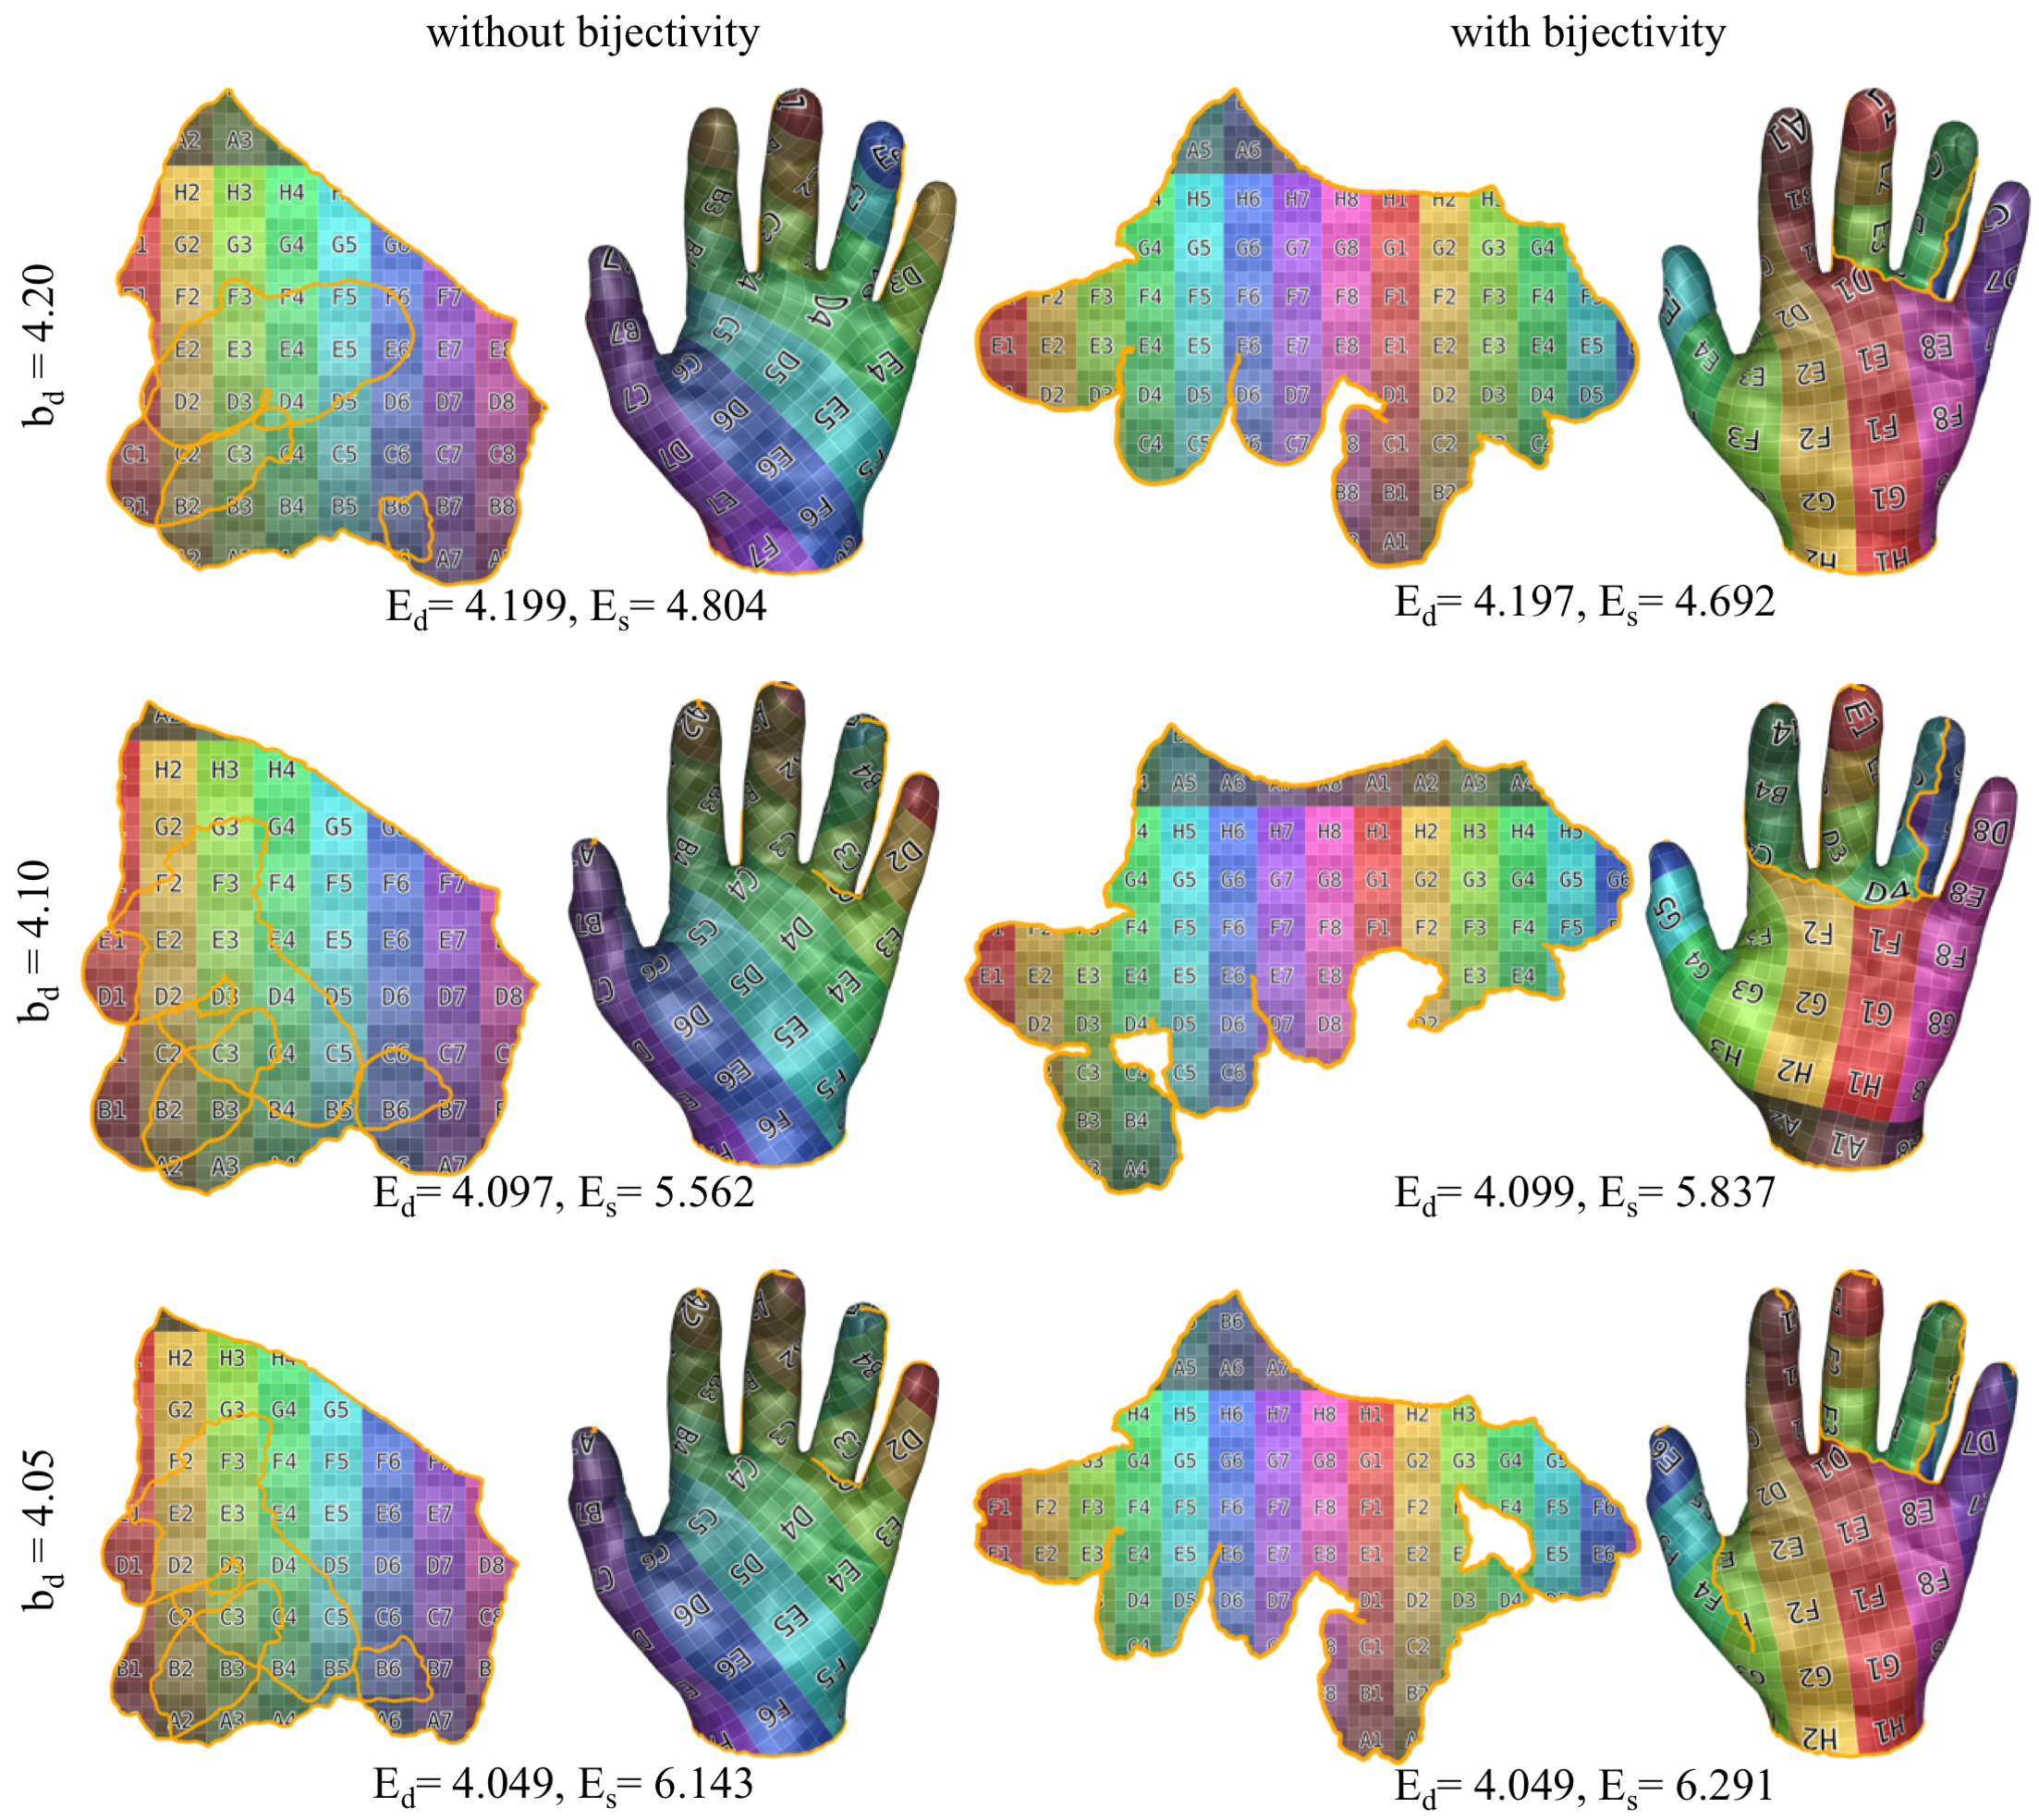
\includegraphics[width=\linewidth]{fig/our_impressive_results_left.png}
\caption{UV maps generated for the hand model by OptCuts both without (left) and with (right) bijectivity enforcement enabled, as we vary the distortion bound $b_d$ over $4.2$, $4.1$, and $4.05$ respectively from top to bottom.}
\label{fig:ours_various_bounds}
\end{figure}

\section{Evaluation}
\label{sec:results}

%We evaluate with a benchmark containing a diverse set of 71 surfaces commonly used in geometry processing research. Meshes in this benchmark are organic shapes with intricate geometric details composed of 81 to 10068 vertices, and are topological disks or spheres \vova{add higher genus if we have it}. In addition, we stress-test the scalability of various methods on a Lucy model that has 48k vertices at the highest resolution.
%We tested our approach on a benchmark containing a diverse set of 71 surfaces commonly used in geometry processing research.  The meshes from this benchmark  are organic shapes with intricate geometric details composed of 81 to 10068 vertices, and are topological disks or spheres \vova{add higher genus if we have it}. In addition, we stress-test the scalability of various methods on a Lucy model that has 48k vertices at the highest resolution.

In the following sections we evaluate OptCuts and a range of other UV parameterization methods and commercial tools on meshes from a benchmark mesh dataset containing a diverse range of 71 surfaces commonly employed in geometry processing research. Meshes in this benchmark are organic shapes with intricate geometric details and varying resolutions ranging from 80 to 10K vertices; we also employ a set of refined Lucy models with resolutions increasing from 2.5K to 48K vertices.

For all examples reported in all of the following sections we note that OptCuts always successfully converges and so achieves the targeted symmetric Dirichlet energy distortion bound $b_d$. Thus in many experiments we will focus on evaluating the seam length measure, $E_{s}$, as an evaluation metric with the goal being to achieve any set target distortion bound with the shortest possible seam lengths. Recall that our seam-length measure, $E_{s}$, is normalized by square root of mesh area and so provides a consistent and comparable measure across examples and methods. 

All our evaluations in the following sections employ our implementation of OptCuts using the libigl~\cite{libigl} library for rapid prototyping and testing. Implementation details are reported above in Section~\ref{sec:imp}. We will release our implementation publicly for future development and application. All experiments presented in this paper were executed on a Macbook Pro with 3.1 GHz quad-core Intel Core i7 CPU and 16 GB 2133 MHz LPDDR3 memory.

%We implement our methods based on libigl\ \cite{libigl} and test it on a Macbook Pro with 3.1 GHz quad-core Intel Core i7 CPU and 16 GB 2133 MHz LPDDR3 memory.
% @misc{libigl,
%   title = {{libigl}: A simple {C++} geometry processing library},
%   author = {Alec Jacobson and Daniele Panozzo and others},
%   note = {http://libigl.github.io/libigl/},
%   year = {2017},
% }

\begin{table}[t]
\centering
\caption{Seam length and performance statistics for our OptCuts algorithm applied to our benchmark of 71 surfaces as we decrease the distortion bound, $b_d$; each example is run with and without our additional enforcement of global bijectivity enabled. All examples converge satisfying the requested distortion bound.}
\label{tb:stats_OptCuts}
\begin{tabular}{|c|c|ccc|ccc|}
\hline
\multirow{2}{*}{$b_d$} & \multirow{2}{*}{bijectivity} & \multicolumn{3}{c|}{$E_{s}$} & \multicolumn{3}{c|}{time (s)} \\ \cline{3-8} 
                       &                         & avg      & min     & max      & avg       & min    & max      \\ \hline
\multirow{2}{*}{4.2}   & OFF                    & 3.819   & 0.080  & 14.545  & 87.0   & 0.3 & 417.8 \\
                       & ON                & 4.087   & 0.289  & 17.063  & 190.3   & 3.8 & 983.3  \\ \hline
\multirow{2}{*}{4.1}   & OFF                    & 4.709   & 0.752  & 17.980  & 137.5  & 0.9 & 886.9 \\
                       & ON                & 5.324   & 0.860  & 21.595  & 271.1   & 6.9 & 1767.8  \\ \hline
\multirow{2}{*}{4.05}  & OFF                    & 6.142   & 0.277  & 21.566  & 213.2  & 3.9 & 1398.1   \\
                       & ON                & 7.195   & 0.932  & 29.596  & 412.9   & 7.2 & 2859.5 \\ \hline
\end{tabular}
\end{table}


\subsection{OptCuts Evaluation}

%\minchen{Add energy plot to show convergence?}

%We directly use our normalized seam length $E_{s}$ as the evaluation metric as it is both shape aware and mesh independent. For comparisons, we always generate UV maps under the same distortion bound either set equally or obtained from the output that are compared with.
%Moreover, this metric also fits in well with practical scenarios where the control of distortions are more intuitive to the users and as-short-as-possible seams are expected.

%We begin by evaluating OptCuts on a benchmark mesh dataset containing a diverse range of 71 surfaces commonly employed in geometry processing research. Meshes in this benchmark are organic shapes with intricate geometric details and varying resolutions ranging from 81 to 10,068 as well as on a set of Lucy models with resolutions increasing from 2.5k to 48k vertices.
%vertices; all are topological disks or spheres \vova{add higher genus if we have it}. In addition, we stress-test the scalability of various methods on a Lucy model that has 48k vertices at the highest resolution.

We first execute OptCuts on our full set of benchmark examples over a range of decreasing target distortion bounds, $b_d \in \{4.2, 4.1, 4.05\}$. For each bound we run OptCuts twice---in each of its modes: once with the global bijectivity constraint enabled, and once with just local-injectivity, i.e. with bijection disabled. As discussed, for all examples in the benchmark, at all three distortion bounds, and both with and without bijectivity constraints, OptCuts always converges to a locally minimal seam length satisfying the prescribed distortion bound. See Figures\ \ref{fig:ours_various_bounds} and \ref{fig:our_impressive_results} for examples of our results as we vary these terms and see our Supplemental materials for a detailed table and visualization of all our OptCuts results, as well as animations of the OptCuts iterations, on the benchmark set. In Table~\ref{tb:stats_OptCuts} we summarize statistics for OptCuts on the benchmark set and observe that as we increase constraint on the examples by tightening distortion bounds and/or enforcing additional bijectivity constraints, longer seams at convergence and comparably longer running times result as expected; see also Figure~\ref{fig:ours_various_bounds}.

%We observe that more constraints such as a tighter distortion bound or global bijectivity necessitate longer seams (Figure~\ref{fig:ours_various_bounds}) and increase computational cost (Table~\ref{tb:stats_OptCuts}).

%We evaluate our method with/without global bijectivity by running them on 70 input surfaces including both disk-topology and closed surfaces (some are with \minchen{[TODO] high genus}), setting $b_d$ to $4.2$, $4.1$, and $4.05$ (Table~\ref{tb:stats_OptCuts}). Our methods automatically generate high quality UV maps given any distortion bounds for all inputs without any user assistance ().


%
\begin{figure}[t]
\centering
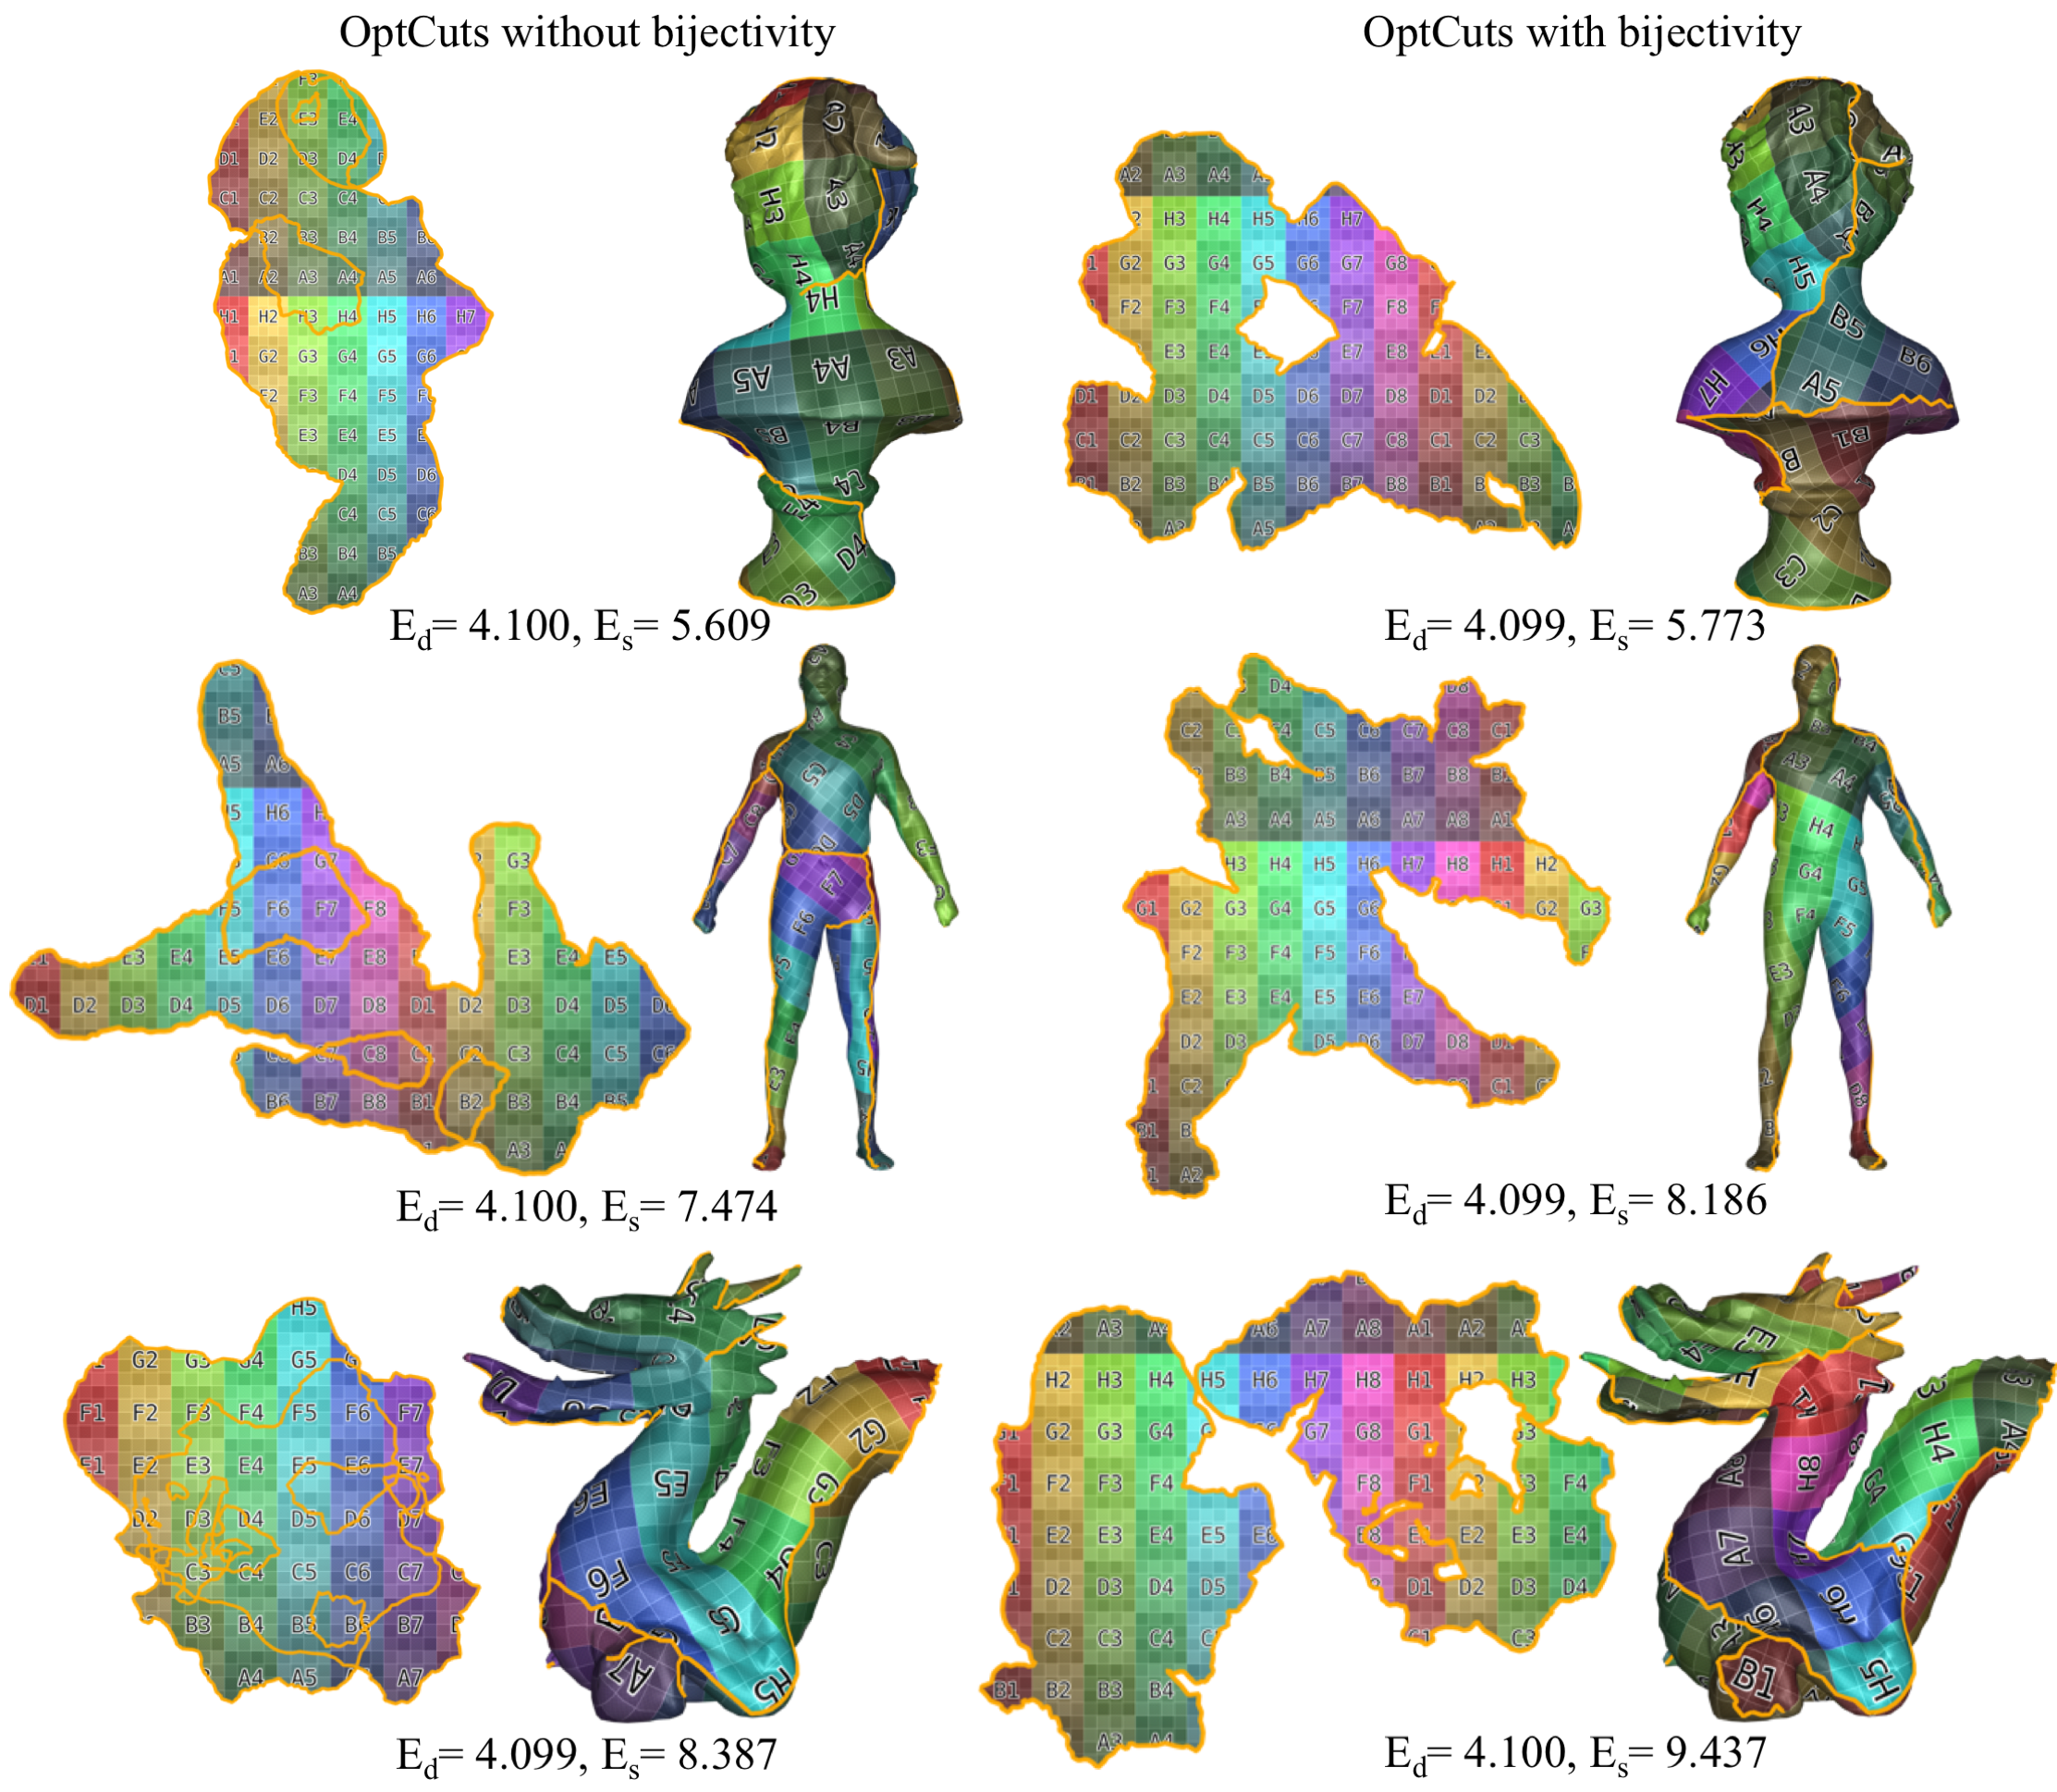
\includegraphics[width=\linewidth]{fig/our_impressive_results_right.png}
\caption{UV maps generated by OptCuts both without (left) and with (right) bijectivity enforcement enabled with the distortion bound set to $b_d$ = $4.1$.}
\label{fig:our_impressive_results}
\end{figure}

%could also be bunny_i, statue_5, wooden_fish


\subsection{Comparisons to AutoCuts}

As discussed in Section~\ref{sec:related}, AutoCuts~\cite{Poranne2017Autocuts} couples the optimization of a weighted sum of a seam-penalty term that tries to pull triangles together, scaled by a scalar $\lambda$, and the symmetric-Dirichlet distortion energy for parameterization. AutoCuts runs in two modes: one interactively driven by direct user guidance throughout, and the second is fully automated. To recreate the automated-mode version of AutoCuts we began with the official AutoCuts implementation and, with guidance from the authors of AutoCuts, set the parameters for recreating their fully automated method to those that performed best across the full set of benchmark examples. 

Recall that in the AutoCuts model the topology of the UV mesh does not change: it remains a triangle soup. Instead, the seam-penalty energy that pulls triangles together is parameterized by a $\delta$ parameter which indicates how far vertices must be from one another to be considered truly disconnected by a seam. Finding a single weighting $\lambda$ that works well for all geometries poses a challenge and likewise $\delta$ requires adjustment over iterations depending on the current stage of the optimization. Thus AutoCuts is generally most effective in interactive mode with a user in-the-loop. For instance, starting from a disconnected triangle soup, a user will gradually decrease $\delta$ defining a {\em homotopy path} over the course of optimization to arrive at a final set of seams. The user also needs to move parameterized components to guide the UV layout towards a globally bijective solution. 

\begin{figure}[h!]
\centering
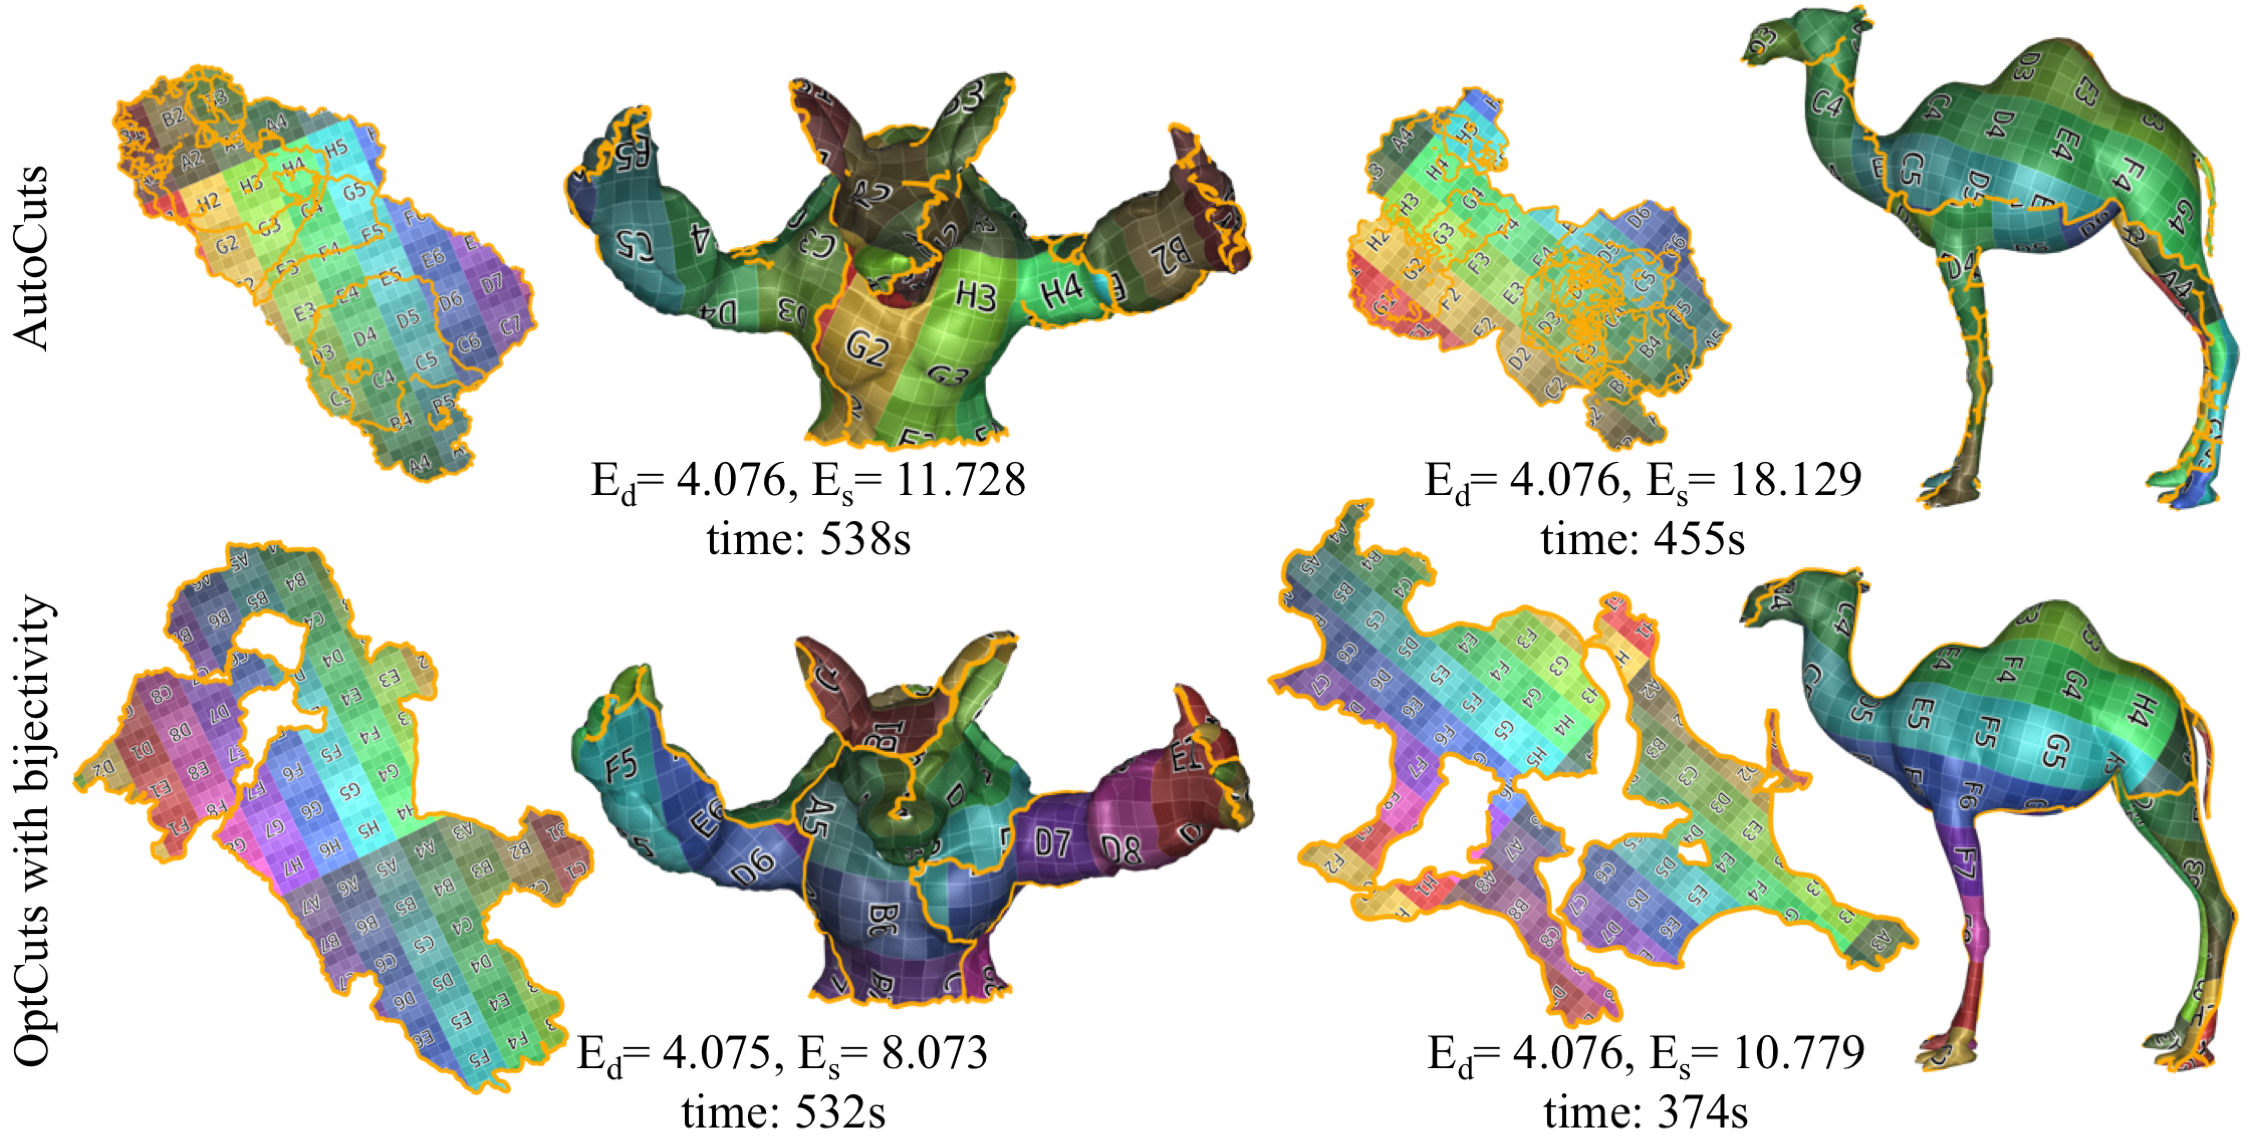
\includegraphics[width=\linewidth]{fig/comp_AutoCuts.png}
\caption{Comparisons between parameterizations generated by AutoCuts (top) and OptCuts with bijectivity enabled (bottom) on Armadillo (left) and Camel (right) model. Here OptCuts obtains improved  seam length measures for the same distortion bound while maintaining additional bijectivity constraints.}
\label{fig:comp_AutoCuts}
\end{figure}
% could also be bone_noInput, bunny_i_f10000, bunny, camel_vova_f10000, cat_noUV, cow_param_closed, dilo, horse, male_2, octopus, wooden_fish, foot_i_f10000, three_man_statue, gargoyle, rgb_dragon, statue_i_1, vase, venus


Thus, the key step in formulating the automated mode for AutoCuts is in automating the homotopy path. This is a prescribed sequence of updates to $\delta$ with ideally a uniform set of mesh-adaptive parameters. In final we set the Autocut parameter $\lambda = 0.4$ and start with $\delta_0=100\overline{e}^2$. We then half this value at the start of each homotopy iteration $\delta_i = \frac{1}{2}\delta_{i-1}$ until it reaches $\delta_\text{term}=10^{-4}\overline{e}^2$. Inside each homotopy iteration, we detect convergence by setting a tolerance $\sqrt{3n_t}\times10^{-3}\overline{e}$ on the $L^2$ norm of UV coordinate changes. Here $\overline{e}$ is the characteristic value of the average edge length in the mesh while $n_t$ is the number of triangles---we seek to make these automated measures robust over varying mesh-resolutions as well as scale.

\danny{Minchen: take a close look at the description above to make sure there are no mistakes. especially on user controls.}
%\vova{using the integer $n_t$ here seems a bit weird... can we explain this choice a bit more?}
%\minchen{This makes the tolerance more invariant to mesh resolution. Imagine two meshes with same $\overline{|e|}$ but $100$ vertices and $100M$ vertices respectively...}

Recall that while AutoCuts enables control of distortion indirectly, it can not and does not guarantee that it will achieve a particular distortion bound. Thus, we perform a re-analysis to gain an understanding of the comparable performance and quality of AutoCuts and OptCuts. We first run automated-mode AutoCuts on each example in the benchmark data set to termination. For each of the examples we then set the resulting distortion measure from the AutoCuts output as the target bound $b_d$ for OptCuts. Here we run OptCuts both with and without global-bijectivity constraints enabled, recalling that, when automated, AutoCuts does not provide bijectivity enforcement. 

As summarized in Table~\ref{tb:comp_AutoCuts}, both versions of OptCuts, both without bijectivity and \emph{with} bijectivity require less time to on average to generate UV maps that have significantly shorter seam lengths than AutoCuts, while achieving the same targeted level of distortion. See  Figure~\ref{fig:comp_AutoCuts} for visual comparisons and our Supplemental for details of all comparison examples. In Figure~\ref{fig:ESLBar_compAutoCuts} we provide a more detailed breakdown of the seam-length comparison for each model in the benchmark with bars sorted by total seam length. 
%Note that methods with longer total seam-length tend to yield longer seams.
\danny{Minchen: for the King Kong (10002 vertices) we have the data that OptCuts only needs 393.6s and 850.7s without/with bijectivity, but AutoCuts needs 1858s; can you add the same info for cathead (131 vertices)? Can you also give the two seam lengths for each example?}
%\vova{Minchen, would be good to say a few words about 2 shapes where our method produces slightly longer seams.} 
%\minchen{It's the kingkong (10002 vertices) and cathead (131 vertices). For kingkong we only need 393.6s and 850.7s without/with bijectivity, but AutoCuts needs 1858s.}\justin{maybe show these in a figure?}\danny{This seems like a good thing to do.}

\paragraph{Scalability}
AutoCuts in both automated and user-guided modes duplicates all vertices in the UV mesh. We observe that this has a significant impact on scalability. Here we analyze how vertex count effects run-time (and implicitly) memory on our full benchmark data-set in Figure~\ref{fig:time_res_compAutoCuts}, and over the Lucy meshes with increasing resolution in Figure~\ref{fig:time_res_compAutoCuts}b. This breakdown of the experiments largely repeats our observations from above that both modes of OptCuts generally outperform AutoCuts while providing better seam-length measures. Here there are two added observations. First, as mesh resolution increases, the performance gap between AuotCuts and OptCuts increases. Second, for moderately large examples, e.g., the two higher resolution Lucy models, at 24k and 48k vertices respectively, the official AutoCuts implementation is already out of memory for both automated and user-guided modes, with their system already $6\times$ larger upon initialization. On the other hand AutoCuts increases vertex counts slowly along cuts and likewise actively seeks to reduce seam lengths and thus extraneous duplicated vertices that would increase system size beyond the initial mesh.

%\minchen{e.g. data points not enough for fitting a trend; for input with 24200 vertices, system size of AutoCuts would be $24200 \times 2 \times 3 \times 2 = 290400$ v.s. $24200 * 2 = 48400$ of OptCuts; ...}

\paragraph{Comparison to interactive-mode AutoCuts and Sorkine et al.\ \shortcite{BoundedDistortParam:2002}}
Finally, in Figure\ \ref{fig:comp_AutoCuts_Olga} we repeat a comparison with Sorkine et al.'s parameterization \ \shortcite{BoundedDistortParam:2002} and the interactive-mode AutoCuts example created to compare with it from Poranne et al.\ \shortcite{Poranne2017Autocuts}, Figure 11. 
%Here we execute OptCuts, with bijectivity constraints, on this example, setting the distortion bound ($b_d$) to match the distortion achieved in the AutoCut user assisted output.
Here we run OptCuts, with bijectivity constraints enabled, setting its distortion bound ($b_d$) to match the distortion achieved by the interactive user assisted AutoCuts output. We observe that OptCuts, Figure\ \ref{fig:comp_AutoCuts_Olga}d), right, then automatically achieves improved seam-length over the interactively created AutoCuts example, Figure\ \ref{fig:comp_AutoCuts_Olga}d) middle, as well as that of Sorkine et al.\ \shortcite{BoundedDistortParam:2002}, Figure\ \ref{fig:comp_AutoCuts_Olga}d) left, and the automated-mode AutoCuts (not shown here).

%%%%%%%%%%%%%%%%%%

% 
%
%
%We compare our method to AutoCuts~\cite{Poranne2017Autocuts}, the state-of-the-art tool that jointly considers cutting and parameterization. 
%They optimize a sum of a seam penalty (weighted by $\lambda$) and a distortion measure. In their formulation, the topology of the mesh does not change
%(it is always a triangle soup), but the seam penalty is parameterized by $\delta$ parameter which indicates how far the vertices have to be from one another
%to be considered disconnected by a seam. Finding a single weight $\lambda$ that fits all geometries poses a challenge, and the parameter
%$\delta$ needs to be adjusted over time depending on the current stage of optimization. Thus, their method is the most effective with the user in the loop. For instance, starting with a disconnected triangle soup, the user gradually decreases $\delta$ defining a {\em homotopy path} over the course of optimization to arrive at a final set of seams. The user also needs to move parameterized components to guide the UV layout towards a globally bijective solution. 
%%
%\vova{take a close look at the description above to make sure there are no mistakes. especially on user controls.}
%
%%
%We used the publicly-available implementation of AutoCuts with guidance from the authors to rebuild the fully automatic version of their method that performed well on our benchmark.  The main challenge lies in constructing appropriate homotopy paths (i.e., the sequence of updates to $\delta$) with a uniform set of mesh-adaptive parameters. In this experiment, we set $\lambda = 0.4$ and started with $\delta_0=100\overline{|e|}^2$; we half this value at the beginning of each homotopy iteration $\delta_i = \frac{1}{2}\delta_{i-1}$ until it reaches $\delta_\text{term}=10^{-4}\overline{|e|}^2$. Inside each homotopy iteration, we detect convergence by setting a tolerance $\sqrt{3n_t}\times10^{-3}\overline{|e|}$ on the $L^2$ norm of UV coordinate changes. Here $\overline{|e|}$ is the average edge length, $n_t$ is the number of triangles.
%%
%\vova{using the integer here seems a bit weird... can we explain this choice a bit more?}
%\minchen{This makes the tolerance more invariant to mesh resolution. Imagine two meshes with same $\overline{|e|}$ but $100$ vertices and $100M$ vertices respectively...}
%
%%
%%AutoCuts obtains high quality UV maps by involving users into the optimization loop. However, when aiming for convenient, fully-automatic methods, the non-smoothness of their Separation energy not only makes it challenging for global parameter settings, but also often end up the optimization with suboptimal results. To show that we automatically generate high quality UV maps without suffering from these issues, we compare our method with a fully automatic version of AutoCuts obtained under the guidance of AutoCuts authors by constructing appropriate homotopy paths with a uniform set of mesh-adaptive parameters. 
%%Specifically, we used $\lambda = 0.4$ and started with $\delta=100\overline{|e|}^2$ and half it in the beginning of each homotopy iteration until it reaches $10^{-4}\overline{|e|}^2$. Inside each homotopy iteration, we detect convergence by setting a tolerance $\sqrt{3n_t}\times10^{-3}\overline{|e|}$ on the $L^2$ norm of UV coordinate changes. Here $\overline{|e|}$ is the average edge length, $n_t$ is the number of triangles.
%
%AutoCuts enables the user to control distortion indirectly by adjusting $\lambda$ parameter, but does not guarantee reaching a particular bound. Thus, to make our comparisons fully automatic we first run AutoCuts on an input surface, and then set the distortion measure for the AutoCuts output as the target bound $b_d$ for our method. Since automatic version of AutoCuts does not naturally support global bijectivity the most direct comparison is to the non-bijective version of our method, but we compare to both variants for completeness.  As demonstrated in Table~\ref{tb:comp_AutoCuts}, both versions of our method require less time to generate UV maps with significantly shorter seams while reaching the same level of distortion. Figure~\ref{fig:ESLBar_compAutoCuts} provides a more detailed comparison for every model in the benchmark:  The bar charts are sorted by total seam length, where methods with longer bars tend to yield longer seams.
%\vova{Minchen, would be good to say a few words about 2 shapes where our method produces slightly longer seams.} 
%\minchen{It's the kingkong (10002 vertices) and cathead (131 vertices). For kingkong we only need 393.6s and 850.7s without/with bijectivity, but AutoCuts needs 1858s.}\justin{maybe show these in a figure?}
%
%Note that we easily enforced bijectivity (Figure~\ref{fig:comp_AutoCuts}), which is only supported in AutoCuts with user assistance on patch manipulation.
%Since AutoCuts does not intuitively support generating UV maps with a certain level of distortion, we first run AutoCuts on a batch of input surfaces, and then set their output distortions as $b_d$ in our method for each input. As demonstrated in Table~\ref{tb:comp_AutoCuts}, for both the two versions of our method, we require less time to generate UV maps with same level of distortion but significantly smaller seams. Figure~\ref{fig:ESLBar_compAutoCuts} shows a bar chart comparison on the output $E_{s}$ of each input surface. Note that we easily enforced bijectivity (Figure~\ref{fig:comp_AutoCuts}), which is only supported in AutoCuts with user assistance on patch manipulation.

\begin{table}[t]
\centering
\caption{
Distortion, seam length, and performance statistics comparing automated-mode AutoCuts (this provides bijectivity enforcement) and our OptCuts algorithm (both with and without bijectivity constraints enabled) on all input surfaces in our benchmark dataset. For each example we set the OPtCuts target distortion ($b_d$) to the achieved (uncontrollable) AutoCuts output distortion on the same example (ranging from $4.016$ to $4.187$). OptCuts in both modes (without and \emph{with} bijectivity) obtains shorter seam lengths and faster run times when compared to AutoCuts.}
\label{tb:comp_AutoCuts}
% \begin{tabular}{|c|ccc|ccc|}
% \hline
% \multirow{2}{*}{method} & \multicolumn{3}{c|}{$E_{s}$} & \multicolumn{3}{c|}{time (s)} \\ \cline{2-7} 
%                         & avg      & min     & max      & avg      & min    & max       \\ \hline
% AutoCuts                & 7.5789   & 1.2069  & 24.6816  & 499.9    & 4.0    & 2677.0    \\
% OptCuts(B)               & 5.8114   & 0.8979  & 19.7405  & 304.0    & 6.4    & 1267.7     \\
% OptCuts               & 5.3065   & 0.8992  & 16.1329  & 148.7    & 3.1    & 650.9    \\ \hline
% \end{tabular}
\begin{tabular}{|c|c|c|c|c|}
\hline
method                   & bijectivity & avg. $E_{d}$ & avg. $E_{s}$ & avg. time (s) \\ \hline
AutoCuts                 & N/A         & 4.074        & 7.5789       & 499.9         \\ \hline
\multirow{2}{*}{OptCuts} & ON          & 4.073        & 5.8114       & 304.0         \\
                         & OFF         & 4.073        & 5.3065       & 148.7         \\ \hline
\end{tabular}
\end{table}

\begin{figure}[t]
\centering
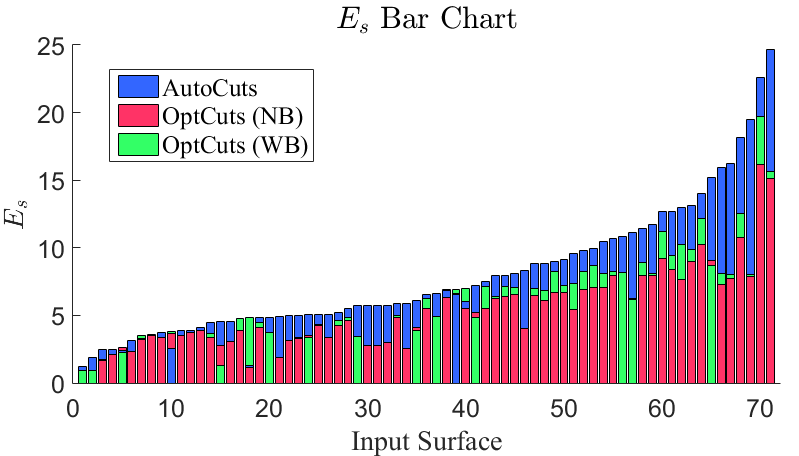
\includegraphics[width=\linewidth]{fig/ESLBar_compAutoCuts.png}
\caption{
A per-example comparison of seam lengths achieved by 
AutoCuts and OptCuts sorted by total seam length. OptCuts without bijectivity constraints in red achieves shorter seams than AutoCuts in blue for all except for two inputs (see text for details on these two examples) while OptCuts with additional bijectivity constraints in green (AutoCuts does not apply bijectvity constraints) still performs favorably in seam length despite the added bijectivity constraints.
%
%\danny{Update caption}Normalized seam length $E_{s}$ bar chart of each example generated by AutoCuts and OptCuts. We (red) achieve shorter seams than AutoCuts (blue) for all except for two inputs, while reaching the same levels of distortion. Our method still performs favorably even with global bijectivity constraints (green).
}
\label{fig:ESLBar_compAutoCuts}
\end{figure}


%\paragraph{Scalability}
%We compare scalability of both methods by analyzing how the vertex count affects the running time. 
%We present this as scatter plot over the benchmark meshes (Figure~\ref{fig:time_res_compAutoCuts}a), 
%and test on a high resolution model of Lucy with 5 different levels of detail (Figure~\ref{fig:time_res_compAutoCuts}b). 
%For higher resolution models (24200 and 48354 vertices) AutoCuts ran out of memory, since their system is $6\times$ 
%larger than ours. For the other models we see that gap between two approaches increases. Since our method 
%adaptively updates the topology of the mesh, we optimize with respect to a smaller number of variables that contributes
%to substantial speedup (since only the vertices along the seam need to be duplicated). 
%%
%\vova{Danny -- I think you had a few other good points about scalability}
%\minchen{e.g. data points not enough for fitting a trend; for input with 24200 vertices, system size of AutoCuts would be $24200 \times 2 \times 3 \times 2 = 290400$ v.s. $24200 * 2 = 48400$ of OptCuts; ...}
%
%%From the time-resolution scatter plot in Figure~\ref{fig:time_res_compAutoCuts}a, we see that for meshes with higher resolution, our method scales better on running time than AutoCuts.
%%We further run AutoCuts and our methods on 5 input surfaces obtained by progressively simplifying the original Lucy model (48354 vertices) to test scalability. From the trend in Figure~\ref{fig:time_res_compAutoCuts}b, we further see that our method scales better. Besides, the average $E_{s}$ obtained by our methods with/without bijectivity on the lucy models are $9.236$ and $8.816$ respectively, much smaller than $13.052$ by AutoCuts. Notice that for models with 24200 and 48354 vertices, AutoCuts already run out of memory, since its system size is $6$ times that of ours.

\begin{figure}[t]
\centering
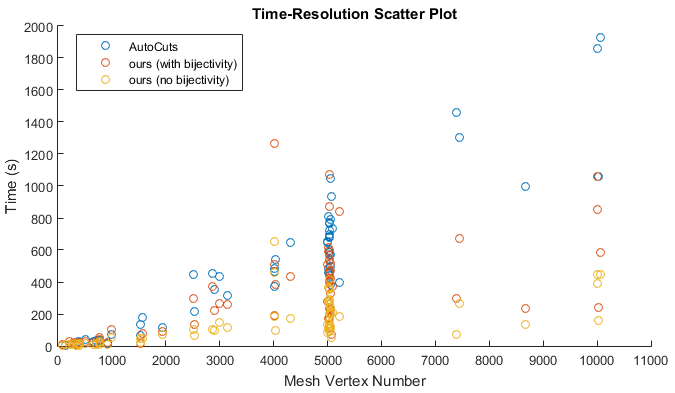
\includegraphics[width=\linewidth]{fig/time_res_compAutoCuts.png}
\caption{Runtime scatterplots for AutoCuts (blue) and OptCuts with bijectivity enforcement (green) and OptCuts without bijectivity (red) across all examples in our benchmark set (left) and for increasing resolutions of the Lucy model (right). Here (left and right) we observe that as mesh resolution increases, the performance gap between AuotCuts and OptCuts increases while (right) for moderately large examples, e.g., the two higher resolution Lucy models, at 24k and 48k vertices respectively, there is no data points for AutoCuts as the official implementation is already out of memory; see our discussion below.
%Both versions of OptCuts require less computation on higher resolution meshes. OptCuts also achieve shorter average seams ($9.236$ with, and $8.816$  without bijectivity) than AutoCuts (13.052), while reaching same target distortion.
}
\label{fig:time_res_compAutoCuts}
\end{figure}


%\paragraph{Global Bijectivity}
%\minchen{In AutoCuts paper, they mentioned in their Figure 11 that they experimented with a greedy procedure based on Sorkine et al.\ \shortcite{BoundedDistortParam:2002} (Figure\ \ref{fig:comp_AutoCuts_Olga}a) to automatically handle bijectivity in AutoCuts (Figure\ \ref{fig:comp_AutoCuts_Olga}b). However, their result with user assisted patch manipulation still ends up with shorter seams (Figure\ \ref{fig:comp_AutoCuts_Olga}c). We execute OptCuts with bijectivity constraints on this example, setting the distortion of their user assisted output as $b_d$. We find that OptCuts achieves shorter seams with bijectivity automatically handled without the need of any user assistance (Figure\ \ref{fig:comp_AutoCuts_Olga}d).}

\begin{figure}[t]
\centering
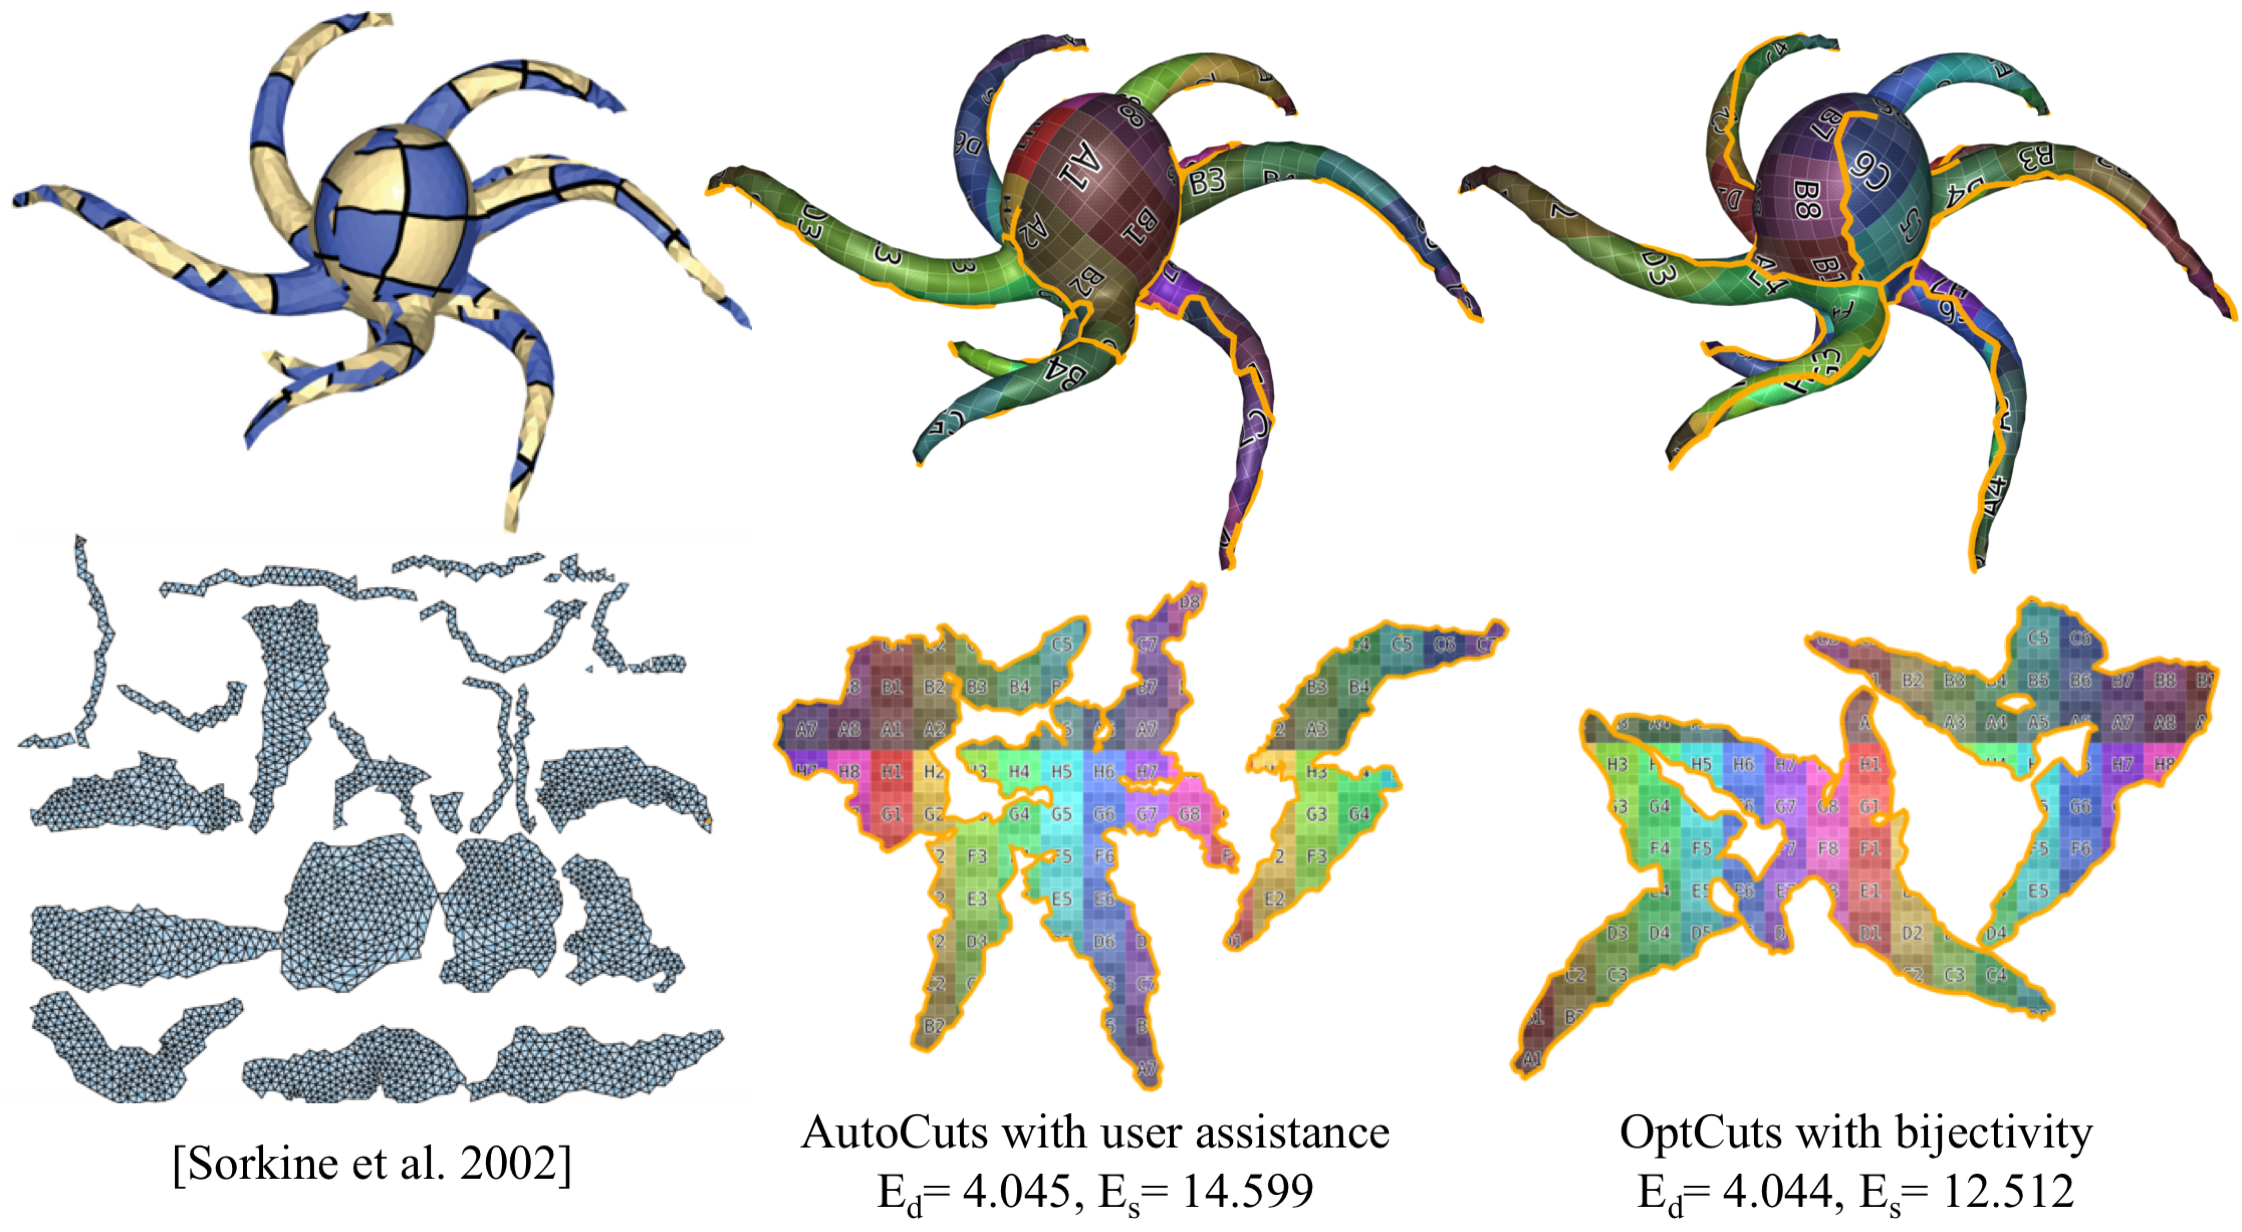
\includegraphics[width=\linewidth]{fig/comp_AutoCuts_Olga.png}
\caption{Here we recreate a comparison with Sorkine et al.'s parameterization \ \shortcite{BoundedDistortParam:2002} (left) and an interactive-mode AutoCuts example created to compare with it from Poranne et al.\ \shortcite{Poranne2017Autocuts} (middle). 
%Here we execute OptCuts, with bijectivity constraints, on this example, setting the distortion bound ($b_d$) to match the distortion achieved in the AutoCut user assisted output.
Right: we run OptCuts with bijectivity constraints enabled, setting its distortion bound ($b_d$) to match the distortion of the interactively user-assisted AutoCuts output. OptCuts satisfies the bound while improving seam-length over the interactively created example.}
\label{fig:comp_AutoCuts_Olga}
\end{figure}


\subsection{Comparison to Commercial Software Tools}
 
Commerical software tools currently offer a range of automated approaches for UV-map creation.
We picked five complex models from our dataset: Lucy, octopus, rgb$\_$dragon, statue$\_$5, and three$\_$man, and asked two experienced artists to create UV maps using the fully automated modes of three commercial software tools: Unwrella\footnote{https://www.unwrella.com/}, ZBrush\footnote{http://pixologic.com/}, and Maya\footnote{https://www.autodesk.com/products/maya/overview}, with default parameter settings. ZBrush generates a single chart UV map and so generally produces higher distortion but lower seam lengths. On the other hand Maya and Unwrella cut the surface into multiple charts to achieve low distortion and efficient packing, generally at the cost of longer seam lengths. ZBrush, and Unwrella in organic mode generally produced best UV maps; the hard-surface mode of Unwrella and Maya both generally cut the surface into many small pieces with very long seams and occasionally produced UV meshes with local inversions and non-manifold vertices. We thus took just the output of ZBrush and Unwrella, in organic mode, for all five examples and then further \emph{improved} them by using their seams to minimize the distortion energy $E_d$. In Table\ \ref{tb:comp_commercial} this is the output we compare OptCuts with for each mesh/tool pairing. In each row we respectively give the distortion and seam measure of each distortion-optimized commercial output, followed by the result obtained by OptCuts when we set the OptCuts distortion bound to match the commercial method's final, optimized distortion. Across all examples for the same level of distortion, we observe that OptCuts obtains shorter seams in eight out of the ten comparisons; see also Figure\ \ref{fig:comp_commercial} for visual comparisons and our Supplemental for all results.


%\minchen{We picked 5 complicated models and asked 2 artists to obtain the UV maps using fully automatic mode of commercial software (Maya\footnote{https://www.autodesk.com/products/maya/overview}, Unwrella\footnote{https://www.unwrella.com/}, and ZBrush\footnote{http://pixologic.com/}) with default parameter setting. Unlike ZBrush that generates a single chart UV map but with relatively higher distortion, Maya and Unwrella cuts the surface into multiple charts to achieve low distortion and efficient packing. However, unless specified organic mode in Unwrella, the hard surface mode of Unwrella together with Maya cut the surface into many small pieces with very long seams. We thus compare our method with ZBrush and Unwrella in organic mode only, first obtaining the distortion bound by using their seams to minimize $E_d$. Under the same level of distortion, we achieve shorter seams in 8 out of the 10 comparisons (Table\ \ref{}). Figure\ \ref{fig:comp_commercial} shows the comparisons on the statue\_5 and rgb\_dragon model.}

%\begin{table*}[t]
%\centering
%\caption{\minchen{Performance of commercial software on 5 input surfaces and OptCuts comparison. Note that for Maya and Unwrella in hard surface mode, the output UV map contains local inversions and non-manifold vertices, thus their $E_d$ showing below are just computed with their output UV map instead of being minimized as for Unwrella in organic mode and ZBrush that we compared with.}}
%\label{tb:comp_commercial}
%\begin{tabular}{|c|cc|cc|cc|cc|cc|cc|}
%\hline
%\multirow{2}{*}{model} & \multicolumn{2}{c|}{Maya} & \multicolumn{2}{c|}{Unwrella HardSurface} & \multicolumn{2}{c|}{Unwrella Organic} & \multicolumn{2}{c|}{OptCuts} & \multicolumn{2}{c|}{ZBrush} & \multicolumn{2}{c|}{OptCuts} \\ \cline{2-13} 
%                       & $E_{d}$     & $E_{s}$     & $E_{d}$               & $E_{s}$              & $E_{d}$            & $E_{s}$            & $E_{d}$                   & $E_{s}$                  & $E_{d}$      & $E_{s}$      & $E_{d}$             & $E_{s}$            \\ \hline
%Lucy                   & 4.268            & 100.209            & 4.136                 & 115.381              & 4.096              & 19.713             & 4.095                     & 10.644                   & 4.258        & 6.635        & 4.257               & 6.520              \\
%octopus                & 4.281       & 72.304      & 4.139                 & 81.328               & 4.071              & 21.723             & 4.069                     & 15.725                   & 4.221        & 14.054       & 4.211               & 14.394             \\
%rgb\_dragon            & 4.269       & 96.370      & 4.140                 & 113.736              & 4.224              & 33.465             & 4.224                     & 16.129                   & 4.743        & 9.249        & 4.743               & 8.633              \\
%statue\_5              & 4.152       & 48.733      & 4.073                 & 53.633               & 4.076              & 14.298             & 4.075                     & 5.092                    & 4.148        & 4.047        & 4.147               & 2.950              \\
%three\_man     & 4.254       & 44.239      & 4.114                 & 46.156               & 4.033              & 19.242             & 4.033                     & 13.457                   & 4.146        & 9.001        & 4.146               & 9.316              \\ \hline
%\end{tabular}
%\end{table*} 

\begin{table*}[t]
\centering
\caption{Summary of distortion and seam-length measures for comparison between five UV-maps created by artists with two commercial tools, Unwrella (organic mode) and ZBrush, and the corresponding results obtained by OptCuts (with bijectvity) when its distortion bound is set to the commercial results' map distortion.}
\label{tb:comp_commercial}
\begin{tabular}{|c|cc|cc|cc|cc|}
\hline
\multirow{2}{*}{model} & \multicolumn{2}{c|}{Unwrella Organic} & \multicolumn{2}{c|}{OptCuts (Unwrella $b_d$)} & \multicolumn{2}{c|}{ZBrush } & \multicolumn{2}{c|}{OptCuts (ZBrush $b_d$)} \\ \cline{2-9} 
                                     & $E_{d}$            & $E_{s}$            & $E_{d}$                   & $E_{s}$                  & $E_{d}$      & $E_{s}$      & $E_{d}$             & $E_{s}$            \\ \hline
Lucy                                 & 4.096              & 19.713             & 4.095                     & 10.644                   & 4.258        & 6.635        & 4.257               & 6.520              \\
octopus                               & 4.071              & 21.723             & 4.069                     & 15.725                   & 4.221        & 14.054       & 4.211               & 14.394             \\
rgb\_dragon                          & 4.224              & 33.465             & 4.224                     & 16.129                   & 4.743        & 9.249        & 4.743               & 8.633              \\
statue\_5                             & 4.076              & 14.298             & 4.075                     & 5.092                    & 4.148        & 4.047        & 4.147               & 2.950              \\
three\_man                            & 4.033              & 19.242             & 4.033                     & 13.457                   & 4.146        & 9.001        & 4.146               & 9.316              \\ \hline
\end{tabular}
\end{table*} 

\begin{figure}[t]
\centering
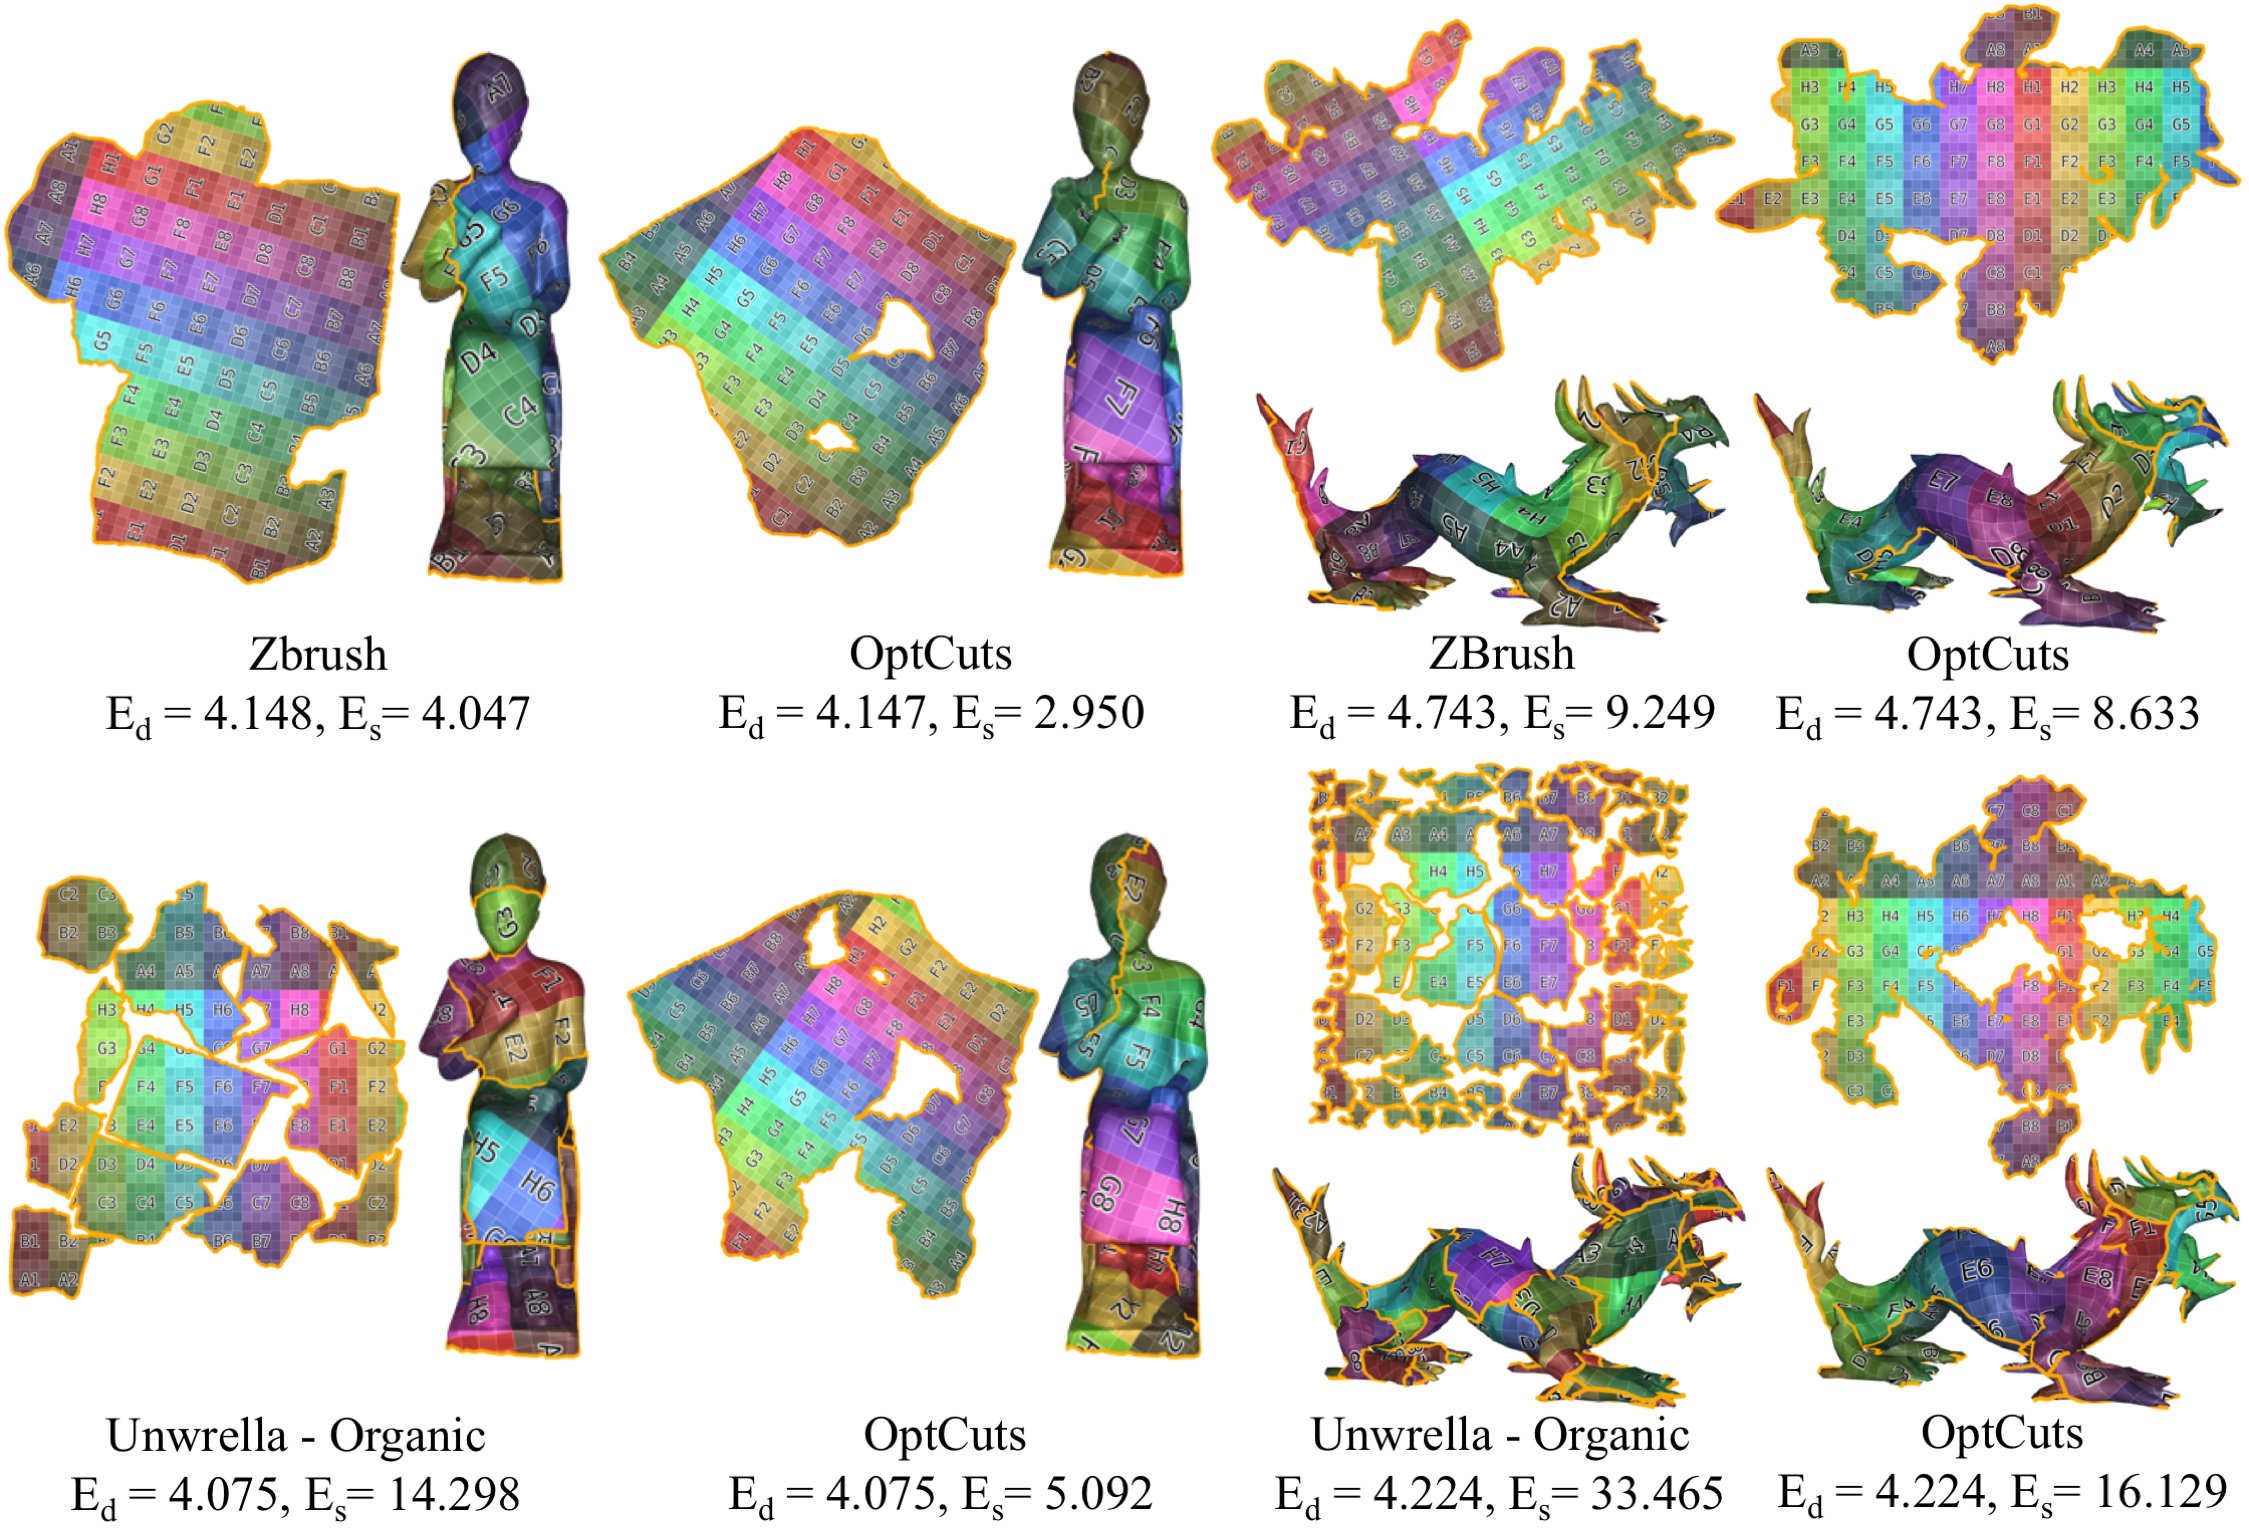
\includegraphics[width=\linewidth]{fig/comp_commercial.png}
\caption{Commercial software tools comparison. Here we compare the results generated by UV-mapping with commercial software tools ZBrush and (top) and Unwrella (bottom) with those obtained by OptCuts with bijectivity constraints enabled. For each comparison example we set OptCuts to match the tools obtained distortion bound, obtaining improved seam measures.
%\danny{Update caption}\minchen{Comparison between commercial software (left, ZBrush at top, Unwrella organic mode at bottom) and OptCuts with bijectivity (right) on the statue\_5 (left) and rgb\_dragon (right) model.
%In this experiment the commercial software are all executed in automatic mode with default parameter setting. Given the seams by ZBrush and Unwrella, we first minimize Symmetric Dirichlet energy and then set the output distortion as $b_d$ in our method. Our method achieved the bound with shorter seams.}
}
\label{fig:comp_commercial}
\end{figure}


\subsection{Variations}
\label{sec:var}
\paragraph{Regional Seam Placement}
Discontinuities produced by seams make texture assignment challenging and can lead to unpleasant rendering artifacts. Thus, UV artists often place seams away from the salient surface regions, e.g., a face. We extend OptCuts to directly enables users to bias or even fully prevent the resulting parameterization from placing cuts in specified regions by painting an intensity weight, $w \in [1.0, +\infty]$ over the three-dimensional surface. As intensities grow we correspondingly penalize the cost of seam lengths in those regions. Correspondingly, in OptCuts we update the seam-length measure by looking up, per-edge $i$, the local painted weight, $w_{i}$, and then simply updating the edge measure to sum to 
\begin{align}
E_s = \frac{1}{\sqrt{(\sum_{t\in\mathcal{F}} |A_t|)/\pi}} \sum_{i \in \mathcal{S}} w_i |e_i|.
\end{align}
%
We demonstrate the results of OptCuts with these additional user-directed constraints in Figure~\ref{fig:regional_seam_placement} bottom, where the user-painted salience map goes from blue with $w = 100$ to green with $w = 1$ in Figure~\ref{fig:regional_seam_placement} middle, and compare with the results obtained from our undirected OptCuts results in Figure~\ref{fig:regional_seam_placement} top. Notice that with the addition of these constraints, OptCuts continues to yield low seam length and to satisfy the distortion bound, but now also enables additional controls on seam placement.
 
%
%In texture painting applications, users would really like regions with the same semantic meanings stay connected or close to each other on the UV map. If we let users to select those regions on the input surface, we could easily avoid seams in those regions while still achieving bijectivity and similar seam length under the same distortion bound (Figure~\ref{fig:regional_seam_placement}). Without changing our framework, we just need to modify our formulation of $E_s$ by weighting each seam edge using the indicator function $w_{s}$ provided by the user:


\begin{figure}[t]
\centering
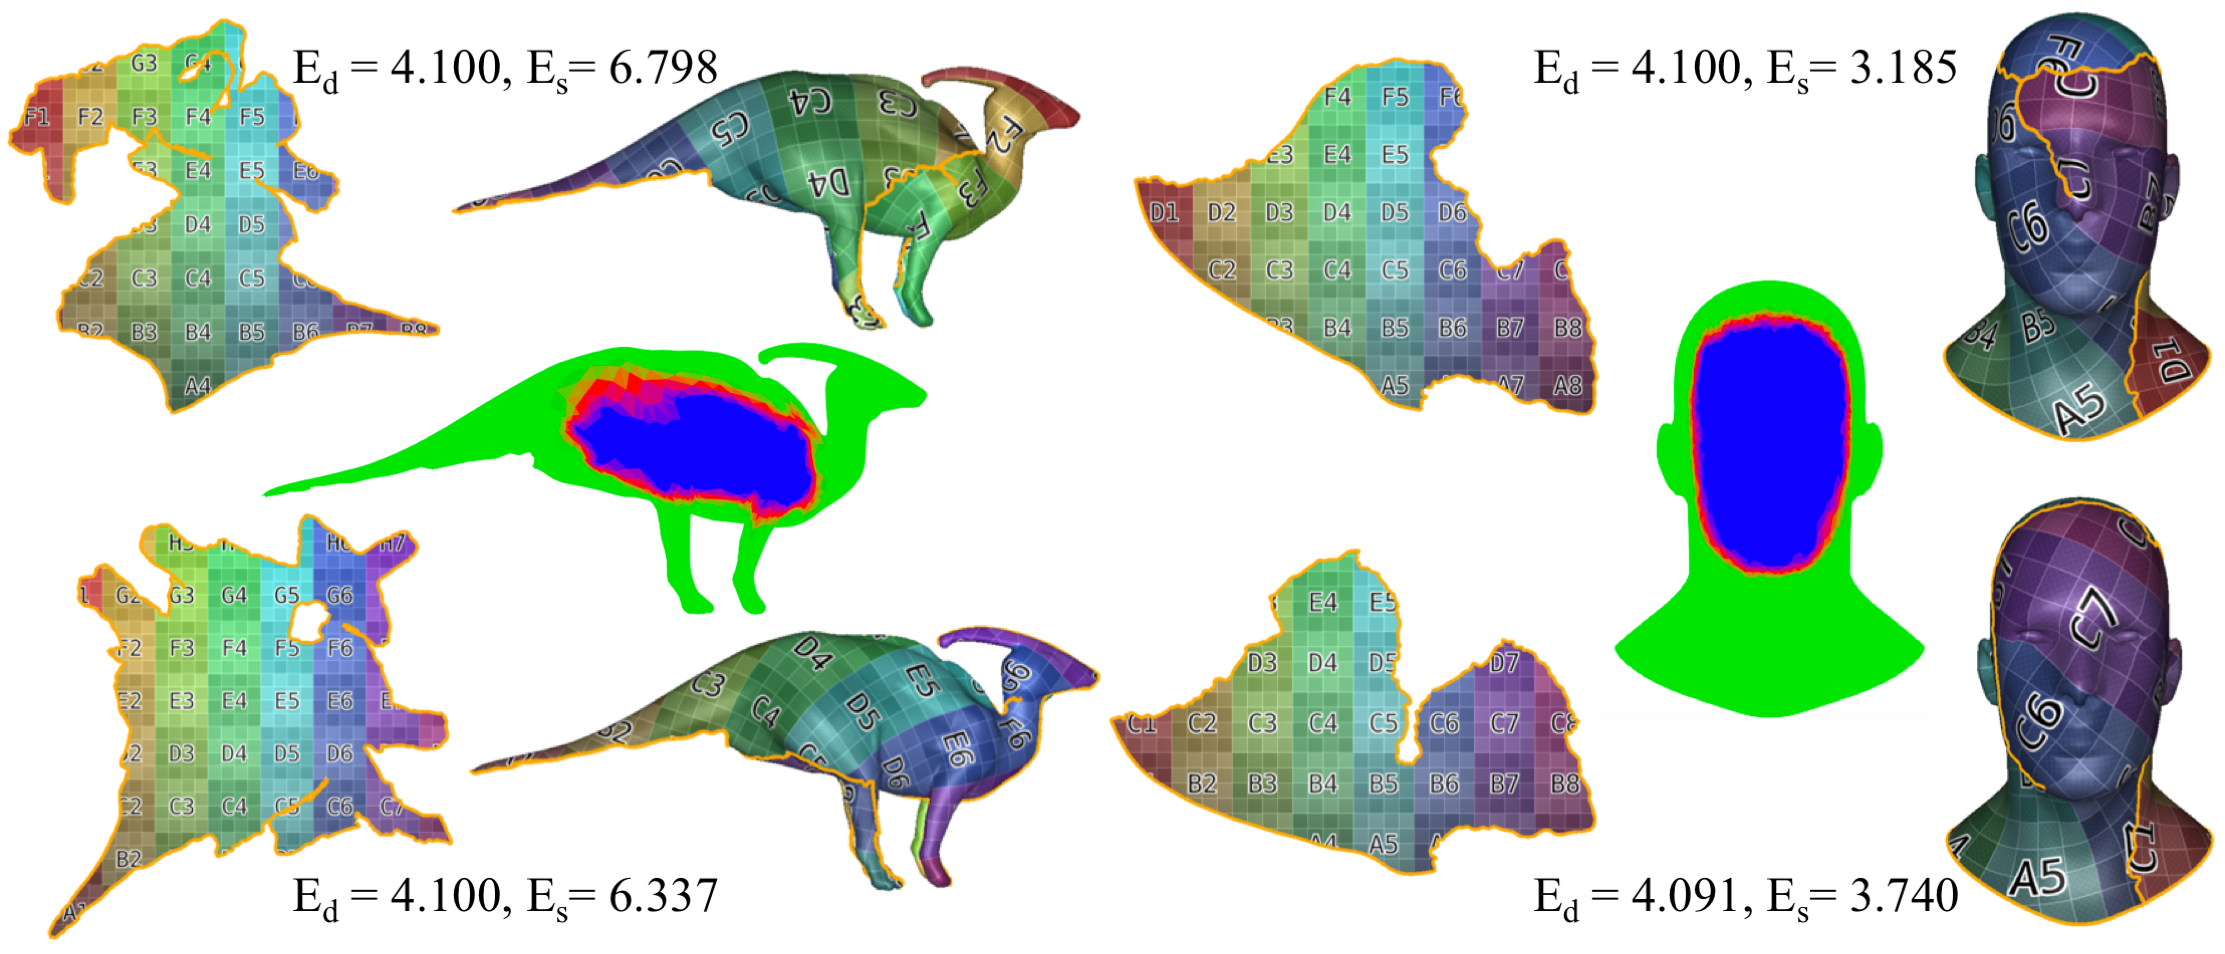
\includegraphics[width=\linewidth]{fig/regional_user.png}
\caption{OptCuts can additionally expose additional constraints allowing 
users to bias or even fully prevent the resulting parameterization from placing cuts in salient regions by painting a map over the three-dimensional surface showing were seams are more or less desirable. 
Middle: a user-painted salience map goes from blue (no seams) to green (seams allowed). With these additional provided constraints OptCuts continues to yield low seam length and to satisfy the distortion bounds while also enables additional controls on seam placement avoiding salient regions(bottom); compare with the results obtained from our undirected OptCuts (bottom). Note as well that here we happen to achieve shorter seams with additional user constraints for the dinosaur model as OptCuts finds local minimizers.}
\label{fig:regional_seam_placement}
\end{figure}

% \paragraph{Conformal Parameterization}
% Using a conformal energy~\cite{Hormann2000MIPS,Sheffer2005ABFPP} for $E_d$ will achieve joint seam placement and conformal parameterization. Figure~\ref{fig:conformal_vs_isometry} shows some results with $E_d = E_{ABForMIPS}$~\cite{} compared to results with $E_d = E_{d}$, where different seams are generated while our framework stays the same.

\paragraph{Alternative Cutting Strategy}
As discussed above our topology descent step leverages a small subset of local topological operations that we have so far found most expressive, efficient and effective. In choosing this subset we experimented with a number of options. In particular we found a subset of more aggressive topological operations taken from Geometry Images~\cite{Gu2002Geometry} very effective. Geometry Images leverages extrema-to-boundary (EB) cuts that connect the current boundary to the most distorted point, under current parameterization, using the shortest geodesic path. The advantage of this cutting strategy in the OptCuts setting is that it introduces more extreme topological updates at each iteration, potentially saving computational effort. We experimented with replacing our topological search in OptCuts with the EB.
 %cutting as before still terminating once $b_d$ is reached). 
 As expected we find that the resulting optimization does indeed converged faster, but we likewise find that the more aggressive EB cutting converges to longer-seam solutions, especially when we seek tighter distortion bounds and when iterations treat nearly-isometric UV maps where extremities are less prominent. See Table~\ref{tb:comp_GI} and Figure~\ref{fig:comp_GI} for a comparison of OptCuts with these two cutting strategies.
%\paragraph{Alternative Cutting Strategy}
%Our topology descent step leverages a small set of local topological operations to keep the framework simple and general. We also reduce the search complexity by filtering the candidates. Alternatively, one can use a richer set of more aggressive topological operations. For example, Geometry Images~\cite{Gu2002Geometry} leverage extrema-to-boundary cuts that connect the current boundary to the most distorted point (under current parameterization) using the shortest geodesic path. The advantage of this strategy is that it introduces more drastic topological updates at each iteration, potentially saving computational effort. We replace our topological search with this strategy (still terminating once $b_d$ is reached) and refer to the resulting variant of our method as EBCuts. As expected we found that the resulting approach is faster, but we found that it yields longer seams especially with tighter distortion bounds (Table~\ref{tb:comp_GI}) and for nearly-isometric UV maps where extremities are less prominent (Figure~\ref{fig:comp_GI}).
%\vova{We used notation $\mathcal{G}_T$ here, I don't think it appeared anywhere in the paper, so I removed it... we can define it earlier and bring it back if necessary...}

%The cutting strategy in the topology descent steps essentially build up the structure of the UV topology graph $\mathcal{G}_T$. By considering local topological operations, we built a dense graph connecting almost all the possible UV topologies and then reduce the search complexity by filtering. Alternatively, one can consider building $\mathcal{G}_T$ using only a sparse set of UV topologies and more aggressive topological operations, like the extremity-boundary (EBCuts) cut applied in Geometry Images~\cite{Gu2002Geometry}.


%We could alternatively apply EBCuts strategy in our framework without bijectivity constraints by simply alternating the cut with distortion minimization processes, and stop right after $b_d$ is reached. This variation of our method reaches identical distortion bounds with very similar seam length compared to our standard method, but is much faster since the EBCuts cut can be decided nearly instantly (Table~\ref{tb:comp_GI}). However, when we set smaller distortion bounds, the quality of the seams by EBCuts cut drops since extremities are not that obvious on a nearly isometric UV map (Figure~\ref{fig:comp_GI}).

\begin{table}[t]
\centering
\caption{
Here we summarize statistics for our benchmark set comparing performance and resulting seam-lengths obtained by our standard OptCuts topology operations as compared with an alternative version of OptCuts employing the more aggressive topology operation of cutting from extrema-to-boundary (EB) from Geometry Images~\cite{Gu2002Geometry}. We run all examples both with and without bijectivity enforcement. As the EB strategy is more aggressive, we observe faster runtimes at the cost of longer seam-lengths.} 
\label{tb:comp_GI}
\begin{tabular}{|c|c|ccc|ccc|}
\hline
\multirow{2}{*}{$b_d$} & \multirow{2}{*}{OptCuts} & \multicolumn{3}{c|}{$E_{s}$} & \multicolumn{3}{c|}{time (s)} \\ \cline{3-8} 
                       &                         & avg      & min     & max      & avg       & min    & max      \\ \hline
\multirow{2}{*}{4.2}   & Standard                    & 3.819   & 0.080  & 14.545  & 87.0   & 0.3 & 417.8 \\
                       & EB                & 3.868   & 0.159  & 14.929  & 13.0   & 0.1 & 72.1  \\ \hline
\multirow{2}{*}{4.1}   & Standard                    & 4.709   & 0.752  & 17.980  & 137.5  & 0.9 & 886.9 \\
                       & EB               & 4.795   & 1.207  & 16.895  & 17.0   & 0.1 & 87.2  \\ \hline
\multirow{2}{*}{4.05}  & Standard                    & 6.142   & 0.277  & 21.566  & 213.2  & 3.9 & 1398.1   \\
                       & EB                & 6.335   & 0.328  & 23.051  & 24.1   & 0.1 & 115.4 \\ \hline
\end{tabular}
\end{table}

\begin{figure}[t]
\centering
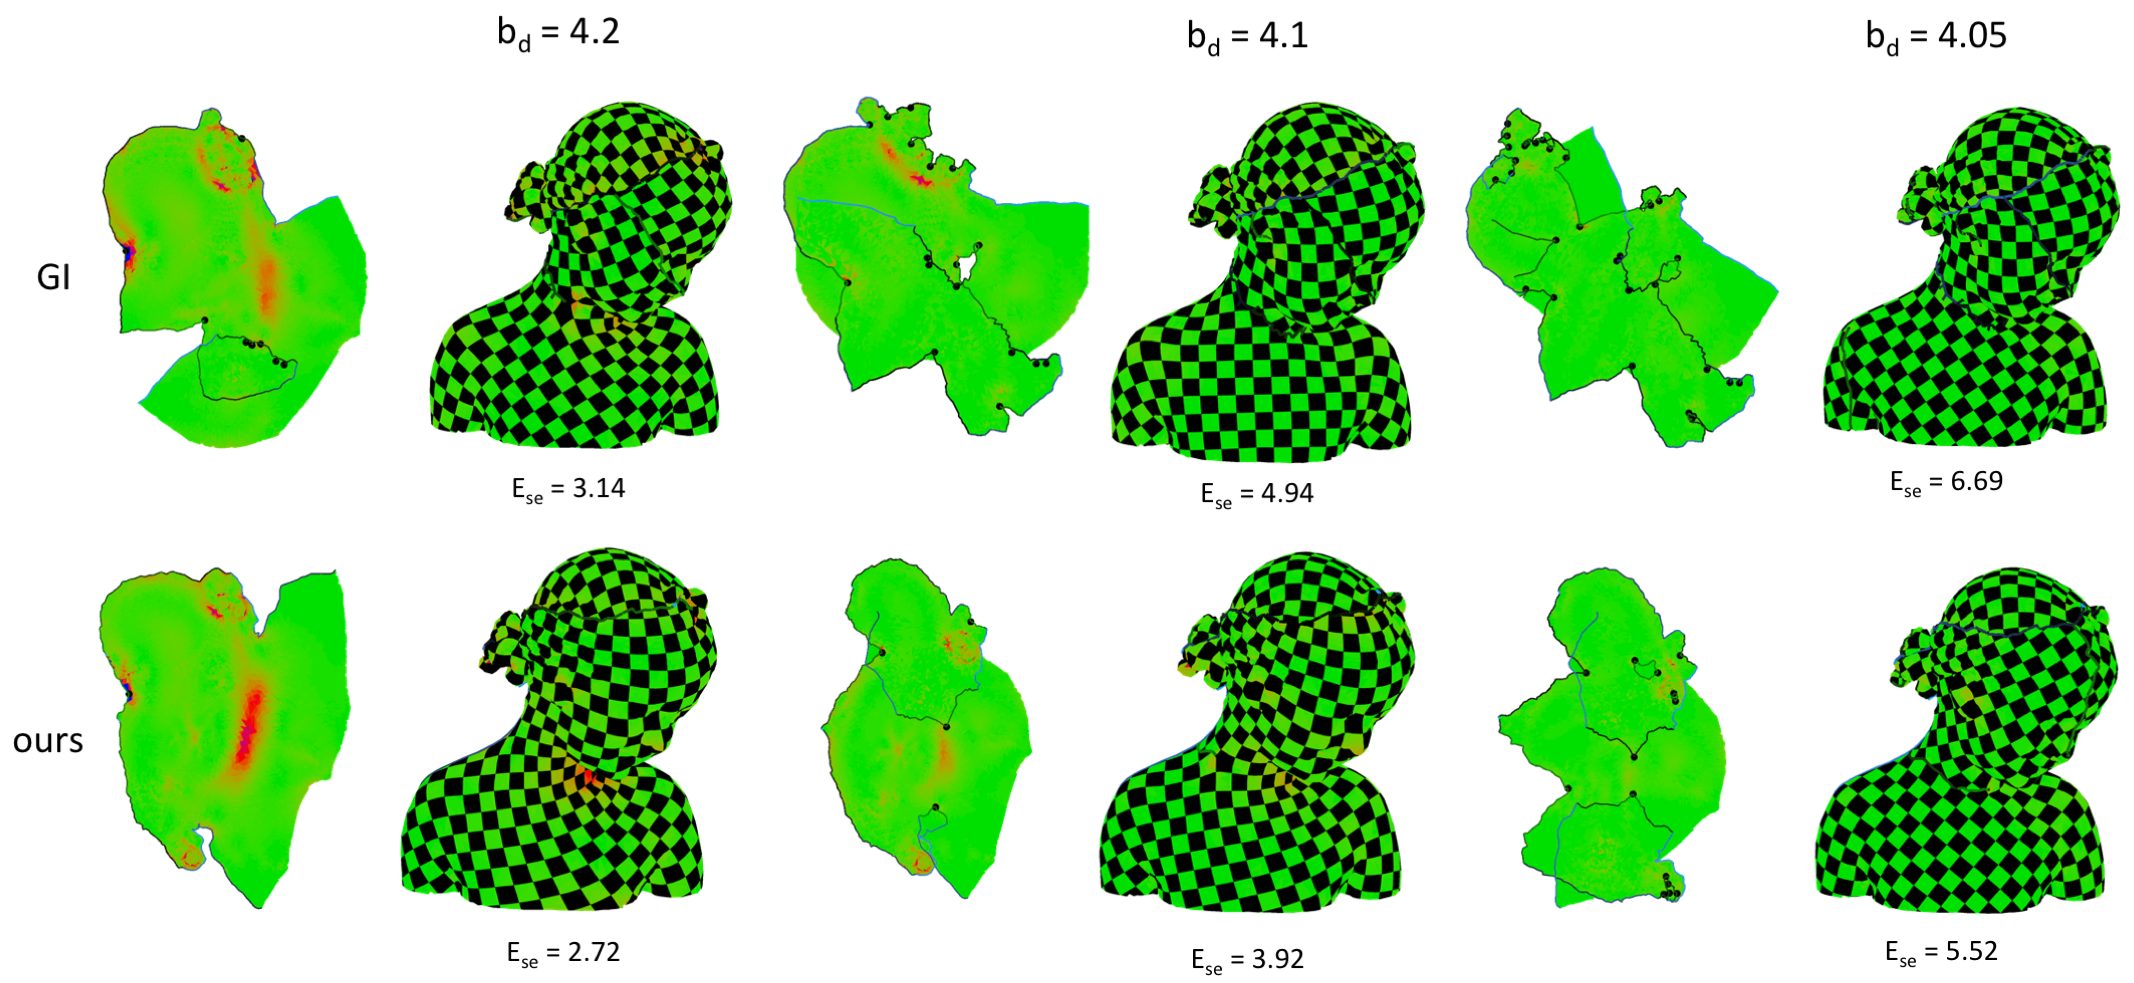
\includegraphics[width=0.8\linewidth]{fig/comp_GI.png}
\caption{Comparisons between OptCuts using our standard topology operations (left), and OptCuts using the extrema-to-boundary (EB) cutting strategy from Geometry Images~\cite{Gu2002Geometry} (right). Here we decrease distortion bounds (top to bottom). EB cuts are aggressive---leading to faster convergence but at the cost of larger seam-length measures at convergence.}
\label{fig:comp_GI}
\end{figure}
% also could be face_f10000, male_body_i_f10000, statue_4_i_f10000, statue_5_i_f10000, bimba_i_f10000

\paragraph{OptCuts Polishing}

In many cases artists and users may have pre-existing UV-mappings, methods and/or pipelines that would benefit from further improvement. Here we observe that OptCuts can take \emph{any} valid embedding as a starting point to improve seam length and/or distortion. To improve just seam length we can set the input map's distortion as an input bound for OptCuts and then optimize the input map for improved seam-length. Alternately, to also improve distortion, we can also apply a lower distortion bound. Likewise, as discussed earlier constrained distortion optimization is highly nonconvex with many local minima; thus polishing multiple warm-started solutions can be an effective way to use OptCuts to explore many interesting locally optimal embeddings.

\danny{I removed the EB example here as it felt possibly confusing as it seemed to be making multiple (and redundant) points here. Minchen: Instead, if time, lets make a few examples polishing the commercial ZBrush outputs.}
%As first example, we take the seams produced by our method with the EBCuts strategy and construct the initial embedding using our standard approach of Tutte's parameterization followed by distortion minimization. We can improve the seam quality while respecting the distortion bound by leveraging our local topological search which enables us to close unnecessary cuts by merging. Even with the bijectivity constraints, we still achieve shorter seam length (Figure~\ref{fig:comp_GI_outputAsInit}). 
%\begin{figure}[t]
%\centering
%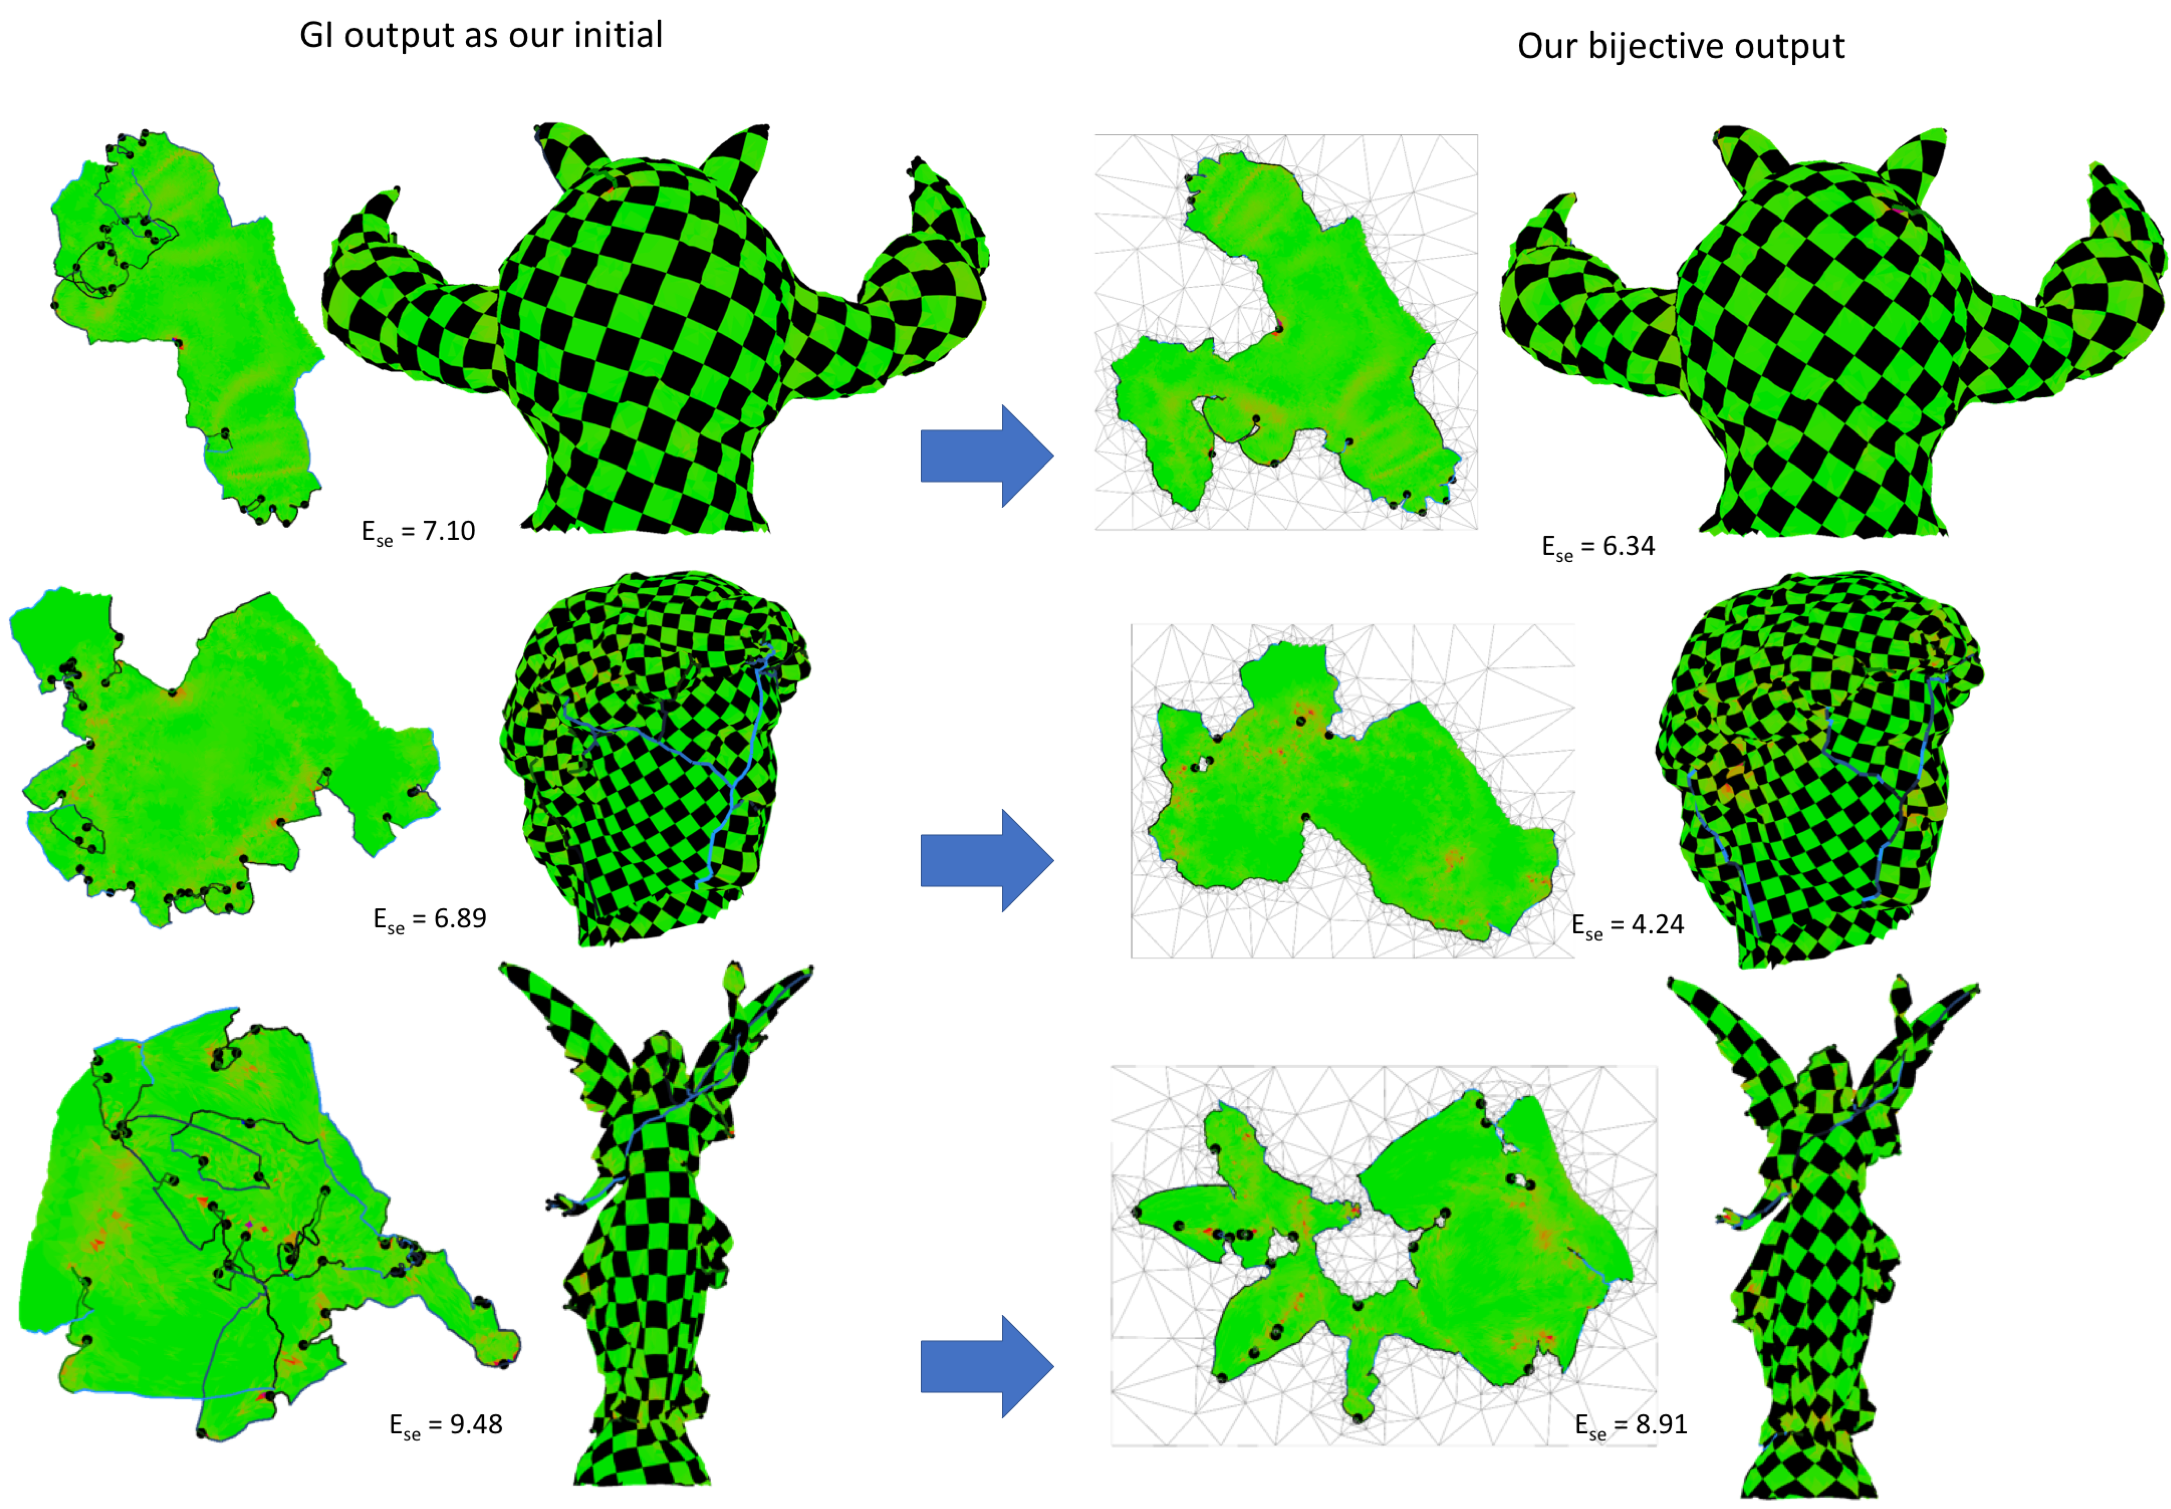
\includegraphics[width=\linewidth]{fig/comp_GI_outputAsInit.png}
%\caption{We use the seams produced by our framework with EBCuts strategy at $b_d = 4.1$  initial UV map (a). We ran our OptCuts framework to improve the seam quality, reaching a locally optimal seam configuration under the given distortion bound even with bijectivity constraints (b). This seam length is also shorter than results obtained by standard OptCuts without bijectivity (c).}
%\label{fig:comp_GI_outputAsInit}
%\end{figure}
% also could be bimba, bunny

Here as an example, we explore taking UV-mappings that are quickly generated by   Seamster~\cite{Sheffer2002Seamster} as input. Seamster is a highly efficient seam cutting strategy that detects local curvature extrema and connects them with a minimal spanning tree. This approach can be sensitive to the user-set parameters such as size of surface regions for computing local extrema, which is a shape-dependent parameter that can require parameter tuning. In this experiment, we pick two models, cow and a triceratops, that have been successfully cut by hand-tuning Seamster\ \cite{Sheffer2002Seamster}. We then apply OptCuts to these two Seamster-generated maps, setting the OptCuts distortion bound to the original distortion of the Seamster-generated maps. In Figure~\ref{fig:comp_Seamster} we compare the original hand-tuned Seamster output in (a), with the resulting OptCuts-polished results in (b), and finally with the direct results of optimizing OptCuts from scratch~\footnote{I.e., directly starting from the Tutte embedding of each mesh.} on these examples while satisfying the same distortion bound in (c). Here the OptCuts-polished examples achieves the shortest seam length while maintaining both the distortion bound and bijectivity---highlighting both the utility of polishing and the value of exploiting warm-starts with OptCuts.


%Since our framework only provides local optima for a highly non-convex problem, initial conditions are relevant for the final result and computational cost. Several powerful topological heuristics have been used to provide a disk topology after cutting. %for the geometry optimization algorithm. 
%We can consider any of these methods as a way to define an initialization for our approach. 

%%%%%%%%%%%%%%%%%%%%%%
%Although we obtain high quality results given any initial embedding, the starting point does affect which local optimal point we will reach. Hence, it is meaningful to explore our method starting from initial seams with global observations. This will also benefit practical scenarios for improving preliminary UV maps while stay close to it.


%As first example, we take the seams produced by our method with the EBCuts strategy and construct the initial embedding using our standard approach of Tutte's parameterization followed by distortion minimization. We can improve the seam quality while respecting the distortion bound by leveraging our local topological search which enables us to close unnecessary cuts by merging. Even with the bijectivity constraints, we still achieve shorter seam length (Figure~\ref{fig:comp_GI_outputAsInit}).
%
%
%The second option we explore is Seamster~\cite{Sheffer2002Seamster}, a classic seam cutting strategy that detects local curvature extrema and connects them with a minimal spanning tree.  This approach can be sensitive to the user-set parameters such as size of surface regions for computing local extrema, which is a shape-dependent parameter that might require tuning. In this experiment, however, we pick two models that have been successfully cut with Seamster (a cow and a triceratops) and use our standard approach to produce the initial embedding, i.e., Tutte's embedding followed by minimizing $E_{d}$ with bijectvitiy constraints (Figure~\ref{fig:comp_Seamster}a). We use the resulting distortion as the upper bound and run the full OptCuts framework on the result. As demonstrated in Figure~\ref{fig:comp_Seamster}b, we achieve shorter seam length while maintaining the distortion bound and bijectivity. This seam length is also shorter than running our standard method without bijectivity from standard initialization (Figure~\ref{fig:comp_Seamster}c).

%With Seamster's best output seams on the cow and triceraptop model, we obtain UV maps by minimizing $E_{d}$ with bijectivity constraints (Figure~\ref{fig:comp_Seamster}a), and use them for warm start, setting their distortions as the upper bounds. As demonstrated in Figure~\ref{fig:comp_Seamster}b, we achieve shorter seam length while maintaining the distortion bound and bijectivity. This seam length is also shorter than running our standard method without bijectivity from standard initialization (Figure~\ref{fig:comp_Seamster}c).
%%%%%%%%%%%%%%%%%%%%%%

\begin{figure}[t]
\centering
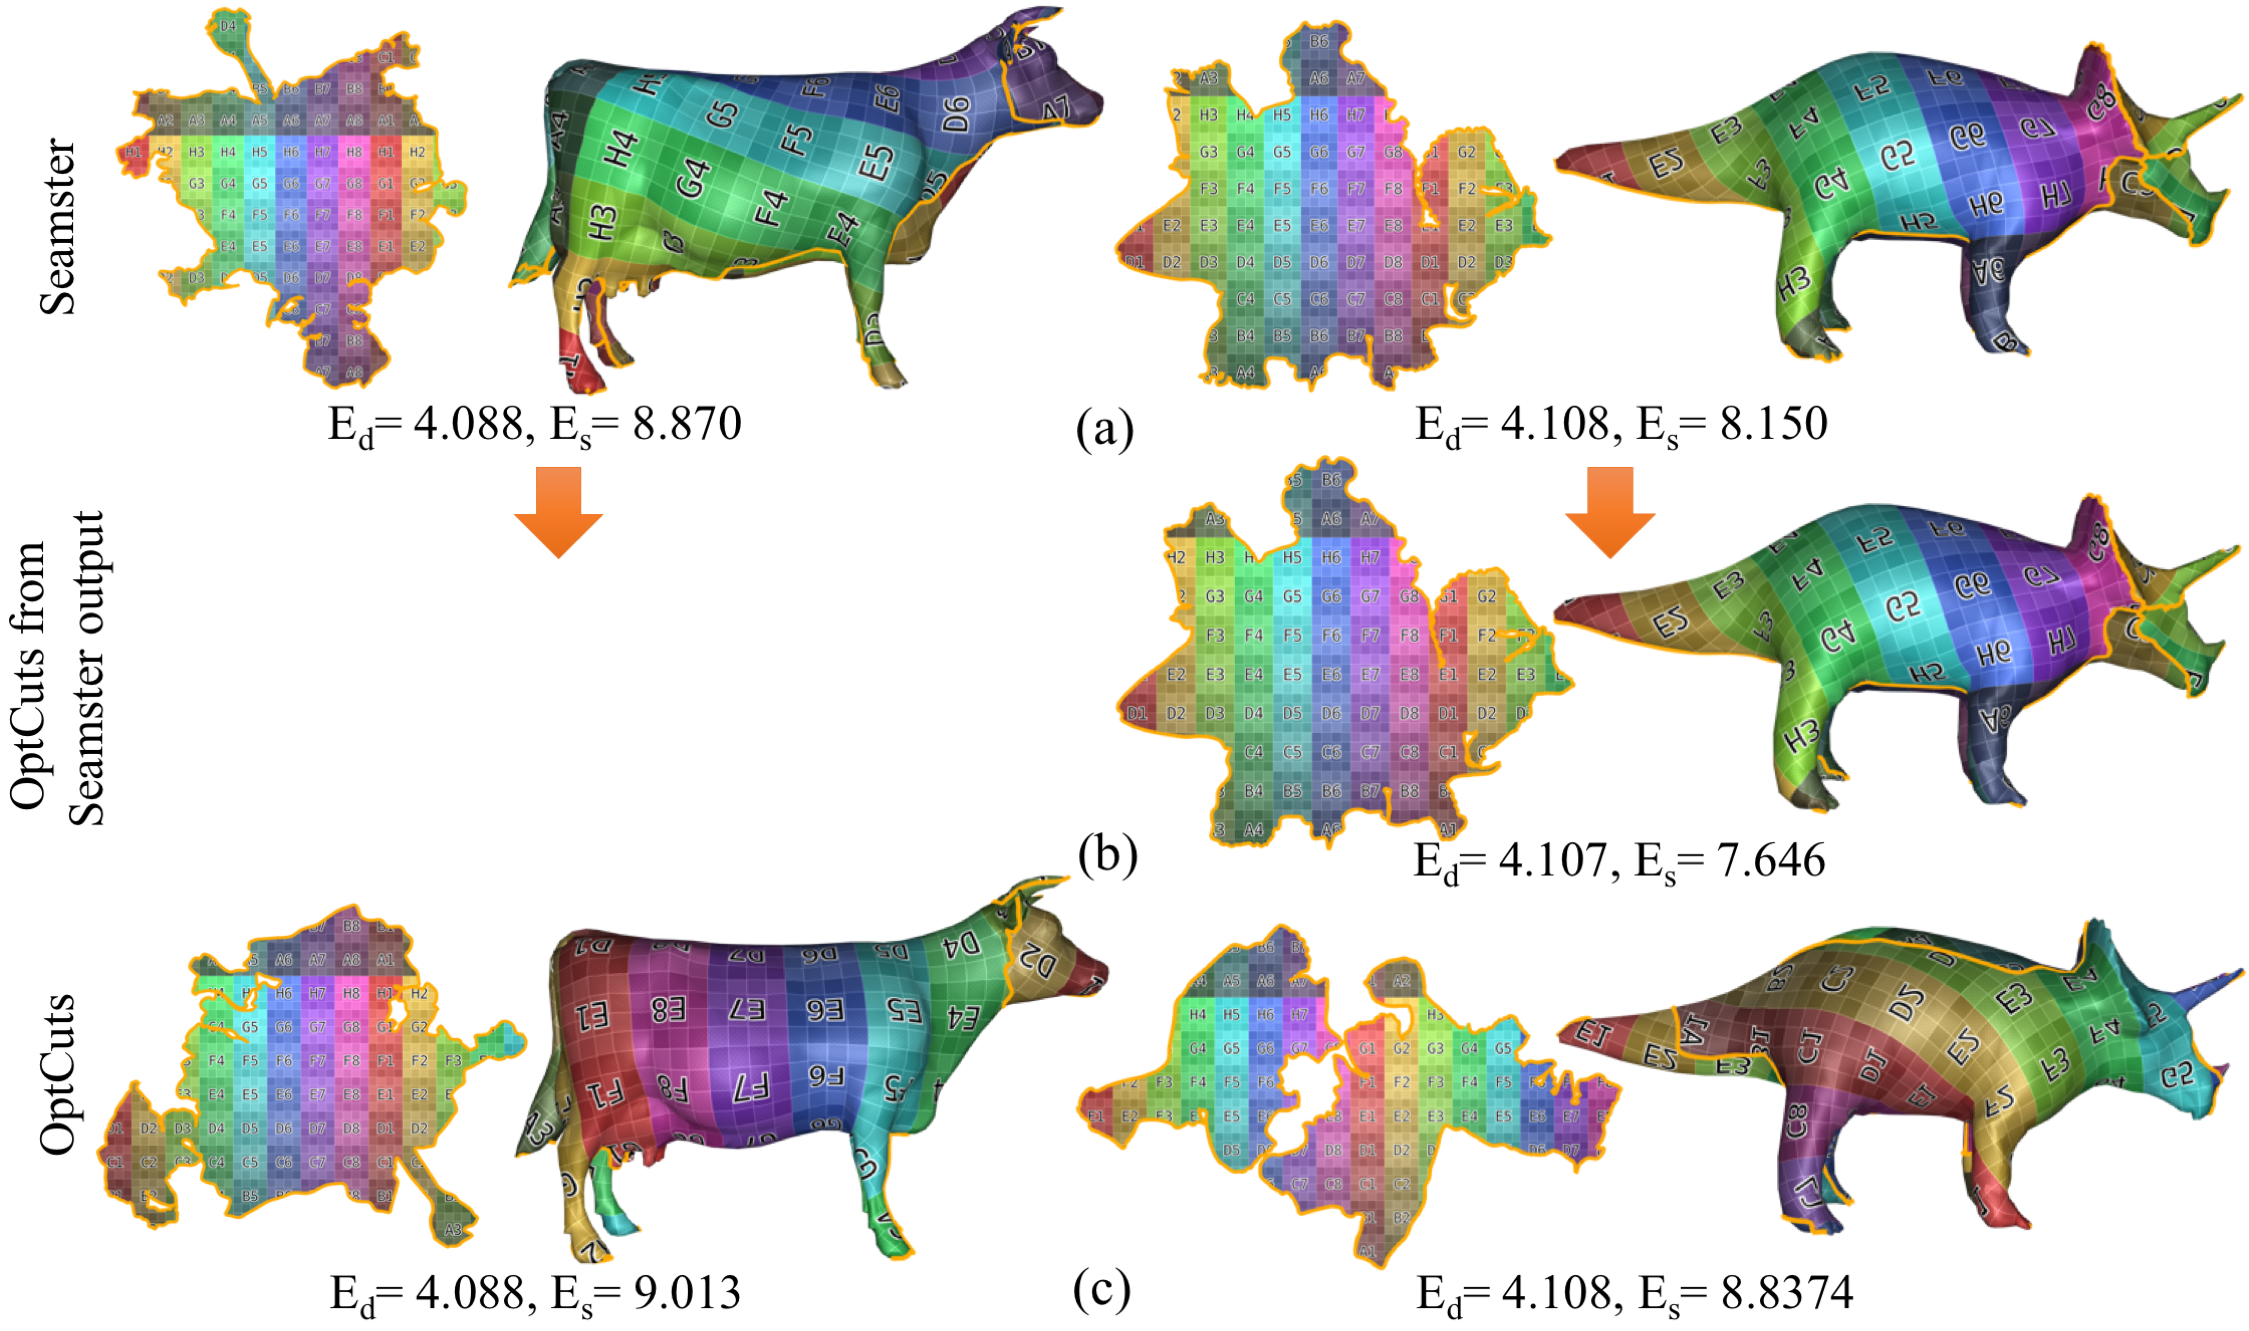
\includegraphics[width=\linewidth]{fig/comp_Seamster.png}
\caption{UV-map Polishing with OptCuts. OptCuts can take \emph{any} valid embedding as a starting point to improve seam length and/or distortion. Here we improve seam length starting from an input map obtained from Seamster\ \cite{Sheffer2002Seamster} (a). We preserve distortion quality while improving seam length by taking the initial map's distortion as an input bound for OptCuts. Then we optimize the input map improving seam length while preserving distortion (b). As constrained distortion optimization is highly nonconvex, with many local minima, polishing warm-started solutions like these can be an effective way to use OptCuts to explore many interesting locally optimal embeddings aside from the default one we gain from initializing with a Tutte embedding (c).}
\label{fig:comp_Seamster}
\end{figure}

%For Seamster, user need to set the size of local regions for measuring extremity, which is a mesh and shape dependent parameter that requires fine tuning. Even OptCuts with standard initialization achieves similar seam length without any user assistance.

